% $Author: oscar $
% $Date: 2009-09-15 16:53:48 +0200 (Tue, 15 Sep 2009) $
% $Revision: 29111 $
%=================================================================
\ifx\wholebook\relax\else
% --------------------------------------------
% Lulu:
	\documentclass[a4paper,10pt,twoside]{book}
	\usepackage[
		papersize={6.13in,9.21in},
		hmargin={.815in,.815in},
		vmargin={.98in,.98in},
		ignoreheadfoot
	]{geometry}
  \usepackage[hangul]{kotex}
	% $Author: oscar $
% $Date: 2009-09-13 20:58:29 +0200 (Sun, 13 Sep 2009) $
% $Revision: 29070 $
%=============================================================
% NB: documentclass must be set in main document.
% Allows book to be generated in multiple formats.
%=============================================================
%:Packages
\usepackage[T1]{fontenc}  %%%%%really important to get the code directly in the text!
\usepackage{palatino}
\usepackage{ifthen}
\usepackage{graphicx}
\graphicspath{{figures/}}
\usepackage{xspace}
\usepackage{makeidx}
\usepackage{isodateo} % enable \isodate
\usepackage{amssymb,textcomp}
%=============================================================
%:More packages
%\usepackage[english]{babel}
%\usepackage{lmodern}
%\usepackage[scaled=0.85]{helvet}
%\usepackage{microtype}
%\usepackage{theorem}
%\usepackage{float}
%\usepackage{longtable}
%\usepackage[nottoc]{tocbibind}
%\usepackage{multicol}
%\usepackage{booktabs}	% book-style tables
%\usepackage{topcapt}	% enables \topcaption
%\usepackage{multirow}
%\usepackage{tabularx}
%\usepackage{alltt}
\usepackage[usenames,dvipsnames]{color}
%\usepackage[hang]{subfigure}\makeatletter\def\p@subfigure{\thefigure\,}\makeatother
%\usepackage{rotating}
%\usepackage{enumitem}	% apb: allows more control over tags in enumerations
%\usepackage{verbatim}     % for comment environment
%\usepackage{varioref}	% for page references that work
%\usepackage{needspace}
%\usepackage[newparttoc]{titlesec}
%\usepackage{titletoc}
%\usepackage{wrapfig}
\usepackage[
	colorlinks=true,
	linkcolor=black,
	urlcolor=black,
	citecolor=black
]{hyperref}   % should come last
%=============================================================
%:URL style
\makeatletter
\def\url@leostyle{%
  \@ifundefined{selectfont}{\def\UrlFont{\sf}}{\def\UrlFont{\sffamily}}}
\makeatother
\urlstyle{leo}
%=============================================================
%:Booleans
\newboolean{lulu}
\setboolean{lulu}{false}
\newcommand{\ifluluelse}[2]{\ifthenelse{\boolean{lulu}}{#1}{#2}}
%=============================================================
%:Editorial comment macros
\newcommand{\nnbb}[2]{
  \fbox{\bfseries\sffamily\scriptsize#1}
  {\sf\small$\blacktriangleright$\textit{#2}$\blacktriangleleft$}
}
\newcommand{\on}[1]{\nnbb{Oscar}{#1}}
\newcommand{\here}{\nnbb{CONTINUE}{HERE}}
%=============================================================
%:Abbreviation macros
\newcommand{\ie}{\emph{i.e.},\xspace}
\newcommand{\eg}{\emph{e.g.},\xspace}
\newcommand{\etc}{\emph{etc.}\xspace}
\newcommand{\etal}{\emph{et al.}\xspace}
\newcommand{\straightquote}{"}
\newcommand{\sba}{\url{SquareBracketAssociates.org}\xspace}
%=============================================================
%:Patterns
% \newcommand{\pattern}[2]{\newpage\section{{\sf #1}}\label{pat:#2}}
% \newcommand{\pattern}[2]{\newpage\index{#1 (Pattern)}\section{#1}\label{pat:#2}}
\newcommand{\pattern}[2]{\cleardoublepage\index{#1 (패턴)}\section{#1}\label{pat:#2}}
\newcommand{\thumbnail}[2]{\index{#1 (패턴)}\subsection{#1}\label{pat:#2}}
\newcommand{\thumblang}[2]{\index{#1 (패턴 랭귀지)}\subsection{#1}\label{pat:#2}}
\newcommand{\variant}[1]{{\emph{#1}}\xspace}
% \newcommand{\problem}[1]{\subsection*{Problem}\emph{#1}}
\newcommand{\intent}[1]{\paragraph{의도}\emph{#1}}
\newcommand{\problem}[1]{\paragraph{문제}\emph{#1}}
\newcommand{\solution}[1]{\paragraph{해결}\emph{#1}}
\newcommand{\discussion}[0]{\paragraph{토론}}
\newcommand{\cmd}[1]{{\tt #1}\xspace}
%=============================================================
%:Environments
\newenvironment{bulletlist}{\begin{itemize}\setlength{\itemsep}{0ex}}
{\end{itemize}}
%=============================================================
%:Cross reference macros
\newcommand{\chalabel}[1]{\label{cha:#1}}
\newcommand{\seclabel}[1]{\label{sec:#1}}
\newcommand{\figlabel}[1]{\label{fig:#1}}
\newcommand{\tablabel}[1]{\label{tab:#1}}
\newcommand{\rulelabel}[1]{\label{rule:#1}}
\newcommand{\eglabel}[1]{\label{eg:#1}}
\newcommand{\scrlabel}[1]{\label{scr:#1}}
\newcommand{\mthlabel}[1]{\label{mth:#1}}
\newcommand{\clslabel}[1]{\label{cls:#1}}
\newcommand{\faqlabel}[1]{\label{faq:#1}}
%\newcommand{\charef}[1]{Chapter~\ref{cha:#1}\xspace}
%\newcommand{\secref}[1]{Section~\ref{sec:#1}\xspace}
\newcommand{\figref}[1]{Figure~\ref{fig:#1}\xspace}
% \newcommand{\patpgref}[2]{\hyperref[pat:#2]{\sf #1} [p.~\pageref{pat:#2}]\xspace}
\newcommand{\patpgref}[2]{\index{#1 (Pattern)}\hyperref[pat:#2]{#1} [p.~\pageref{pat:#2}]\xspace}
\newcommand{\patlangpgref}[2]{\index{#1 (Pattern language)}\hyperref[pat:#2]{#1} [p.~\pageref{pat:#2}]\xspace}
% \newcommand{\patref}[2]{\hyperref[pat:#2]{\sf #1}\xspace}
\newcommand{\patref}[2]{\index{#1 (Pattern)}\hyperref[pat:#2]{#1}\xspace}
\newcommand{\patlangref}[2]{\index{#1 (Pattern language)}\hyperref[pat:#2]{#1}\xspace}
% \newcommand{\charef}[2]{\hyperref[cha:#2]{\underline{\sf #1}}\xspace}
% \newcommand{\charef}[2]{\hyperref[cha:#2]{\sf #1}\xspace}
\newcommand{\charef}[2]{\index{#1 (Pattern cluster)}\hyperref[cha:#2]{#1}\xspace}
% \newcommand{\chapgref}[2]{\hyperref[cha:#2]{\sf #1} [p.~\pageref{cha:#2}]\xspace}
\newcommand{\chapgref}[2]{\index{#1 (Pattern cluster)}\hyperref[cha:#2]{#1} [p.~\pageref{cha:#2}]\xspace}
%\newcommand{\Figref}[1]{Figure~\ref{fig:#1}\xspace}
%\newcommand{\appref}[1]{Appendix~\ref{app:#1}\xspace}
%\newcommand{\tabref}[1]{Table~\ref{tab:#1}\xspace}
%\newcommand{\ruleref}[1]{\ref{rule:#1}\xspace}
%\newcommand{\egref}[1]{example~\ref{eg:#1}\xspace}
%\newcommand{\Egref}[1]{Example~\ref{eg:#1}\xspace}
%\newcommand{\scrref}[1]{script~\ref{scr:#1}\xspace}
%\newcommand{\Scrref}[1]{Script~\ref{scr:#1}\xspace}
%\newcommand{\tscrref}[1]{the script~\ref{scr:#1}\xspace}
%\newcommand{\Tscrref}[1]{The script~\ref{scr:#1}\xspace}
%\newcommand{\mthref}[1]{method~\ref{mth:#1}\xspace}
%\newcommand{\mthsref}[1]{methods~\ref{mth:#1}\xspace}
%\newcommand{\Mthref}[1]{Method~\ref{mth:#1}\xspace}
%\newcommand{\tmthref}[1]{the method~\ref{mth:#1}\xspace}
%\newcommand{\Tmthref}[1]{The method~\ref{mth:#1}\xspace}
%\newcommand{\clsref}[1]{class~\ref{cls:#1}\xspace}
%\newcommand{\tclsref}[1]{the class~\ref{cls:#1}\xspace}
%\newcommand{\Tclsref}[1]{The class~\ref{cls:#1}\xspace}
%=============================================================
%:Page Layout
\setlength{\headsep}{1cm}
%=============================================================
%:Menu item macro
%\definecolor{lightgray}{gray}{0.89}
%\newcommand{\menu}[1]{{%
%	\setlength{\fboxsep}{0pt}%
%	\colorbox{lightgray}{{{\upshape\sffamily\strut \,#1\,}}}}}
%\newcommand{\go}{\,$\triangleright$\,}
%\newcommand{\short}[1]{\mbox{{\sc cmd}\hspace{0.08em}--\hspace{0.09em}#1}\xspace}
%\newcommand{\button}[1]{{%
%	\setlength{\fboxsep}{0pt}%
%	\fbox{{\upshape\sffamily\strut \,#1\,}}}}
%\newcommand{\toolsflap}{\textit{Tools} flap\xspace}
%=============================================================
%:Section depth
%\setcounter{secnumdepth}{2}
%
%\DeclareGraphicsExtensions{.pdf, .jpg, .png}
%=============================================================
%:PDF setup
\hypersetup{
   pdftitle={Object-Oriented Reengineering Patterns},
   pdfauthor={Serge Demeyer, St\'ephane Ducasse, Oscar Nierstrasz},
   pdfkeywords={Reengineering, Object-Oriented Programming, Patterns},
   pdfsubject={Computer Science}
}
%=============================================================
%:Page layout and appearance
%\renewcommand{\chaptermark}[1]{\markboth{#1}{}}
%\renewcommand{\sectionmark}[1]{\markright{\thesection\ #1}}
%\renewpagestyle{plain}[\small\itshape]{%
%	\setheadrule{0pt}%
%	\sethead[][][]{}{}{}%
%	\setfoot[][][]{}{}{}}
%\renewpagestyle{headings}[\small\itshape]{%
%	\setheadrule{0pt}%
%	\setmarks{chapter}{section}%
%	\sethead[\thepage][][\chaptertitle]{\sectiontitle}{}{\thepage}%
%	\setfoot[][][]{}{}{}}
%=============================================================
%:Title section setup and TOC numbering depth
%\setcounter{secnumdepth}{1}
%\setcounter{tocdepth}{1}
%\titleformat{\part}[display]{\centering}{\huge\partname\ \thepart}{1em}{\Huge\textbf}[]
%\titleformat{\chapter}[display]{}{\huge\chaptertitlename\ \thechapter}{1em}{\Huge\raggedright\textbf}[]
%\titlecontents{part}[3pc]{%
%		\pagebreak[2]\addvspace{1em plus.4em minus.2em}%
%		\leavevmode\large\bfseries}
%	{\contentslabel{3pc}}{\hspace*{-3pc}}
%	{}[\nopagebreak]
%\titlecontents{chapter}[3pc]{%
%		\pagebreak[0]\addvspace{1em plus.2em minus.2em}%
%		\leavevmode\bfseries}
%	{\contentslabel{3pc}}{}
%	{\hfill\contentspage}[\nopagebreak]
%\dottedcontents{section}[3pc]{}{3pc}{1pc}
%\dottedcontents{subsection}[3pc]{}{0pc}{1pc}
%\let\origdoublepage\cleardoublepage
%\newcommand{\clearemptydoublepage}{%
%  \clearpage
%  {\pagestyle{empty}\origdoublepage}}
%\let\cleardoublepage\clearemptydoublepage % see http://www.tex.ac.uk/cgi-bin/texfaq2html?label=patch
%=============================================================
%:Listings package configuration
\newcommand{\caret}{\makebox{\raisebox{0.4ex}{\footnotesize{$\wedge$}}}}
% \newcommand{\escape}{{\sf \textbackslash}}
\definecolor{source}{gray}{0.95}
\usepackage{listings}
\lstdefinelanguage{Smalltalk}{
  morestring=[d]',
% Adapt this to other languages!
%  morecomment=[s]{"}{"},
  alsoletter={\#:},
  %escapechar={!},
  literate=
    {BANG}{!}1
%    {UNDERSCORE}{\_}1
    {\\st}{Smalltalk}9 % convenience -- in case \st occurs in code
    % {'}{{\textquotesingle}}1 % replaced by upquote=true in \lstset
%    {_}{{$\leftarrow$}}1
    {>>>}{{\sep}}1
    {^}{{$\uparrow$}}1
    {~}{{$\sim$}}1
    {-}{{\sf -\hspace{-0.13em}-}}1  % the goal is to make - the same width as +
    {+}{\raisebox{0.08ex}{+}}1		% and to raise + off the baseline to match -
    {-->}{{\quad$\longrightarrow$\quad}}3
	, % Don't forget the comma at the end!
  tabsize=4
}[keywords,comments,strings]

\lstset{language=Smalltalk,
	basicstyle=\sffamily,
	keywordstyle=\color{black}\bfseries,
	% stringstyle=\ttfamily, % Ugly! do we really want this? -- on
	mathescape=true,
	showstringspaces=false,
	keepspaces=true,
	breaklines=true,
	breakautoindent=true,
	backgroundcolor=\color{source},
	lineskip={-1pt}, % Ugly hack
	upquote=true, % straight quote; requires textcomp package
	columns=fullflexible} % no fixed width fonts
% \newcommand{\ct}{\lstinline[mathescape=false,basicstyle={\sffamily\upshape}]}
\newcommand{\ct}{\lstinline[mathescape=false,backgroundcolor=\color{white},basicstyle={\sffamily\upshape}]}
\newcommand{\lct}[1]{{\textsf{\textup{#1}}}}
%\newcommand{\scat}[1]{\emph{\textsf{#1}}\xspace}
%\newcommand{\prot}[1]{\emph{\textsf{#1}}\xspace}
% NB: No argument!
\lstnewenvironment{code}[0]{%
	\lstset{%
		% frame=lines,
		frame=single,
		framerule=0pt,
		mathescape=false
	}
}{}
%\def\ignoredollar#1{}
%=============================================================
%:Reserving space
%\newcommand{\needlines}[1]{\Needspace{#1\baselineskip}}
%=============================================================
%:Indexing macros
% Macros ending with "ind" generate text as well as an index entry
% Macros ending with "index" *only* generate an index entry
\newcommand{\ind}[1]{\index{#1}#1\xspace} % plain text
\newcommand{\subind}[2]{\index{#1!#2}#2\xspace} % show #2, subindex under #1
\newcommand{\emphind}[1]{\index{#1}\emph{#1}\xspace} % emph #1
\newcommand{\emphsubind}[2]{\index{#1!#2}\emph{#2}\xspace} % show emph #2, subindex under #1
\newcommand{\patind}[1]{\index{#1@#1 (pattern)}\ct{#1}\xspace} % pattern
\newcommand{\seeindex}[2]{\index{#1|see{#2}}} % #1, see #2
%\newcommand{\boldidx}[1]{{\bf #1}} % breaks hyperlink
%\newcommand{\indmain}[1]{\index{#1}#1\xspace} 
%\newcommand{\emphsubindmain}[2]{\index{#1!#2}\emph{#2}\xspace} % subindex, main entry
%\newcommand{\subindmain}[2]{\index{#1!#2}#2\xspace} % subindex, main entry
%\newcommand{\clsindmain}[1]{\index{#1!\#@(class)}\ct{#1}\xspace} % class main
%\newcommand{\indexmain}[1]{\index{#1}} 
%=============================================================
\parskip 1ex
%=============================================================

	\pagestyle{headings}
	\setboolean{lulu}{true}
% --------------------------------------------
% A4:
%	\documentclass[a4paper,11pt,twoside]{book}
%	% $Author: oscar $
% $Date: 2009-09-13 20:58:29 +0200 (Sun, 13 Sep 2009) $
% $Revision: 29070 $
%=============================================================
% NB: documentclass must be set in main document.
% Allows book to be generated in multiple formats.
%=============================================================
%:Packages
\usepackage[T1]{fontenc}  %%%%%really important to get the code directly in the text!
\usepackage{palatino}
\usepackage{ifthen}
\usepackage{graphicx}
\graphicspath{{figures/}}
\usepackage{xspace}
\usepackage{makeidx}
\usepackage{isodateo} % enable \isodate
\usepackage{amssymb,textcomp}
%=============================================================
%:More packages
%\usepackage[english]{babel}
%\usepackage{lmodern}
%\usepackage[scaled=0.85]{helvet}
%\usepackage{microtype}
%\usepackage{theorem}
%\usepackage{float}
%\usepackage{longtable}
%\usepackage[nottoc]{tocbibind}
%\usepackage{multicol}
%\usepackage{booktabs}	% book-style tables
%\usepackage{topcapt}	% enables \topcaption
%\usepackage{multirow}
%\usepackage{tabularx}
%\usepackage{alltt}
\usepackage[usenames,dvipsnames]{color}
%\usepackage[hang]{subfigure}\makeatletter\def\p@subfigure{\thefigure\,}\makeatother
%\usepackage{rotating}
%\usepackage{enumitem}	% apb: allows more control over tags in enumerations
%\usepackage{verbatim}     % for comment environment
%\usepackage{varioref}	% for page references that work
%\usepackage{needspace}
%\usepackage[newparttoc]{titlesec}
%\usepackage{titletoc}
%\usepackage{wrapfig}
\usepackage[
	colorlinks=true,
	linkcolor=black,
	urlcolor=black,
	citecolor=black
]{hyperref}   % should come last
%=============================================================
%:URL style
\makeatletter
\def\url@leostyle{%
  \@ifundefined{selectfont}{\def\UrlFont{\sf}}{\def\UrlFont{\sffamily}}}
\makeatother
\urlstyle{leo}
%=============================================================
%:Booleans
\newboolean{lulu}
\setboolean{lulu}{false}
\newcommand{\ifluluelse}[2]{\ifthenelse{\boolean{lulu}}{#1}{#2}}
%=============================================================
%:Editorial comment macros
\newcommand{\nnbb}[2]{
  \fbox{\bfseries\sffamily\scriptsize#1}
  {\sf\small$\blacktriangleright$\textit{#2}$\blacktriangleleft$}
}
\newcommand{\on}[1]{\nnbb{Oscar}{#1}}
\newcommand{\here}{\nnbb{CONTINUE}{HERE}}
%=============================================================
%:Abbreviation macros
\newcommand{\ie}{\emph{i.e.},\xspace}
\newcommand{\eg}{\emph{e.g.},\xspace}
\newcommand{\etc}{\emph{etc.}\xspace}
\newcommand{\etal}{\emph{et al.}\xspace}
\newcommand{\straightquote}{"}
\newcommand{\sba}{\url{SquareBracketAssociates.org}\xspace}
%=============================================================
%:Patterns
% \newcommand{\pattern}[2]{\newpage\section{{\sf #1}}\label{pat:#2}}
% \newcommand{\pattern}[2]{\newpage\index{#1 (Pattern)}\section{#1}\label{pat:#2}}
\newcommand{\pattern}[2]{\cleardoublepage\index{#1 (패턴)}\section{#1}\label{pat:#2}}
\newcommand{\thumbnail}[2]{\index{#1 (패턴)}\subsection{#1}\label{pat:#2}}
\newcommand{\thumblang}[2]{\index{#1 (패턴 랭귀지)}\subsection{#1}\label{pat:#2}}
\newcommand{\variant}[1]{{\emph{#1}}\xspace}
% \newcommand{\problem}[1]{\subsection*{Problem}\emph{#1}}
\newcommand{\intent}[1]{\paragraph{의도}\emph{#1}}
\newcommand{\problem}[1]{\paragraph{문제}\emph{#1}}
\newcommand{\solution}[1]{\paragraph{해결}\emph{#1}}
\newcommand{\discussion}[0]{\paragraph{토론}}
\newcommand{\cmd}[1]{{\tt #1}\xspace}
%=============================================================
%:Environments
\newenvironment{bulletlist}{\begin{itemize}\setlength{\itemsep}{0ex}}
{\end{itemize}}
%=============================================================
%:Cross reference macros
\newcommand{\chalabel}[1]{\label{cha:#1}}
\newcommand{\seclabel}[1]{\label{sec:#1}}
\newcommand{\figlabel}[1]{\label{fig:#1}}
\newcommand{\tablabel}[1]{\label{tab:#1}}
\newcommand{\rulelabel}[1]{\label{rule:#1}}
\newcommand{\eglabel}[1]{\label{eg:#1}}
\newcommand{\scrlabel}[1]{\label{scr:#1}}
\newcommand{\mthlabel}[1]{\label{mth:#1}}
\newcommand{\clslabel}[1]{\label{cls:#1}}
\newcommand{\faqlabel}[1]{\label{faq:#1}}
%\newcommand{\charef}[1]{Chapter~\ref{cha:#1}\xspace}
%\newcommand{\secref}[1]{Section~\ref{sec:#1}\xspace}
\newcommand{\figref}[1]{Figure~\ref{fig:#1}\xspace}
% \newcommand{\patpgref}[2]{\hyperref[pat:#2]{\sf #1} [p.~\pageref{pat:#2}]\xspace}
\newcommand{\patpgref}[2]{\index{#1 (Pattern)}\hyperref[pat:#2]{#1} [p.~\pageref{pat:#2}]\xspace}
\newcommand{\patlangpgref}[2]{\index{#1 (Pattern language)}\hyperref[pat:#2]{#1} [p.~\pageref{pat:#2}]\xspace}
% \newcommand{\patref}[2]{\hyperref[pat:#2]{\sf #1}\xspace}
\newcommand{\patref}[2]{\index{#1 (Pattern)}\hyperref[pat:#2]{#1}\xspace}
\newcommand{\patlangref}[2]{\index{#1 (Pattern language)}\hyperref[pat:#2]{#1}\xspace}
% \newcommand{\charef}[2]{\hyperref[cha:#2]{\underline{\sf #1}}\xspace}
% \newcommand{\charef}[2]{\hyperref[cha:#2]{\sf #1}\xspace}
\newcommand{\charef}[2]{\index{#1 (Pattern cluster)}\hyperref[cha:#2]{#1}\xspace}
% \newcommand{\chapgref}[2]{\hyperref[cha:#2]{\sf #1} [p.~\pageref{cha:#2}]\xspace}
\newcommand{\chapgref}[2]{\index{#1 (Pattern cluster)}\hyperref[cha:#2]{#1} [p.~\pageref{cha:#2}]\xspace}
%\newcommand{\Figref}[1]{Figure~\ref{fig:#1}\xspace}
%\newcommand{\appref}[1]{Appendix~\ref{app:#1}\xspace}
%\newcommand{\tabref}[1]{Table~\ref{tab:#1}\xspace}
%\newcommand{\ruleref}[1]{\ref{rule:#1}\xspace}
%\newcommand{\egref}[1]{example~\ref{eg:#1}\xspace}
%\newcommand{\Egref}[1]{Example~\ref{eg:#1}\xspace}
%\newcommand{\scrref}[1]{script~\ref{scr:#1}\xspace}
%\newcommand{\Scrref}[1]{Script~\ref{scr:#1}\xspace}
%\newcommand{\tscrref}[1]{the script~\ref{scr:#1}\xspace}
%\newcommand{\Tscrref}[1]{The script~\ref{scr:#1}\xspace}
%\newcommand{\mthref}[1]{method~\ref{mth:#1}\xspace}
%\newcommand{\mthsref}[1]{methods~\ref{mth:#1}\xspace}
%\newcommand{\Mthref}[1]{Method~\ref{mth:#1}\xspace}
%\newcommand{\tmthref}[1]{the method~\ref{mth:#1}\xspace}
%\newcommand{\Tmthref}[1]{The method~\ref{mth:#1}\xspace}
%\newcommand{\clsref}[1]{class~\ref{cls:#1}\xspace}
%\newcommand{\tclsref}[1]{the class~\ref{cls:#1}\xspace}
%\newcommand{\Tclsref}[1]{The class~\ref{cls:#1}\xspace}
%=============================================================
%:Page Layout
\setlength{\headsep}{1cm}
%=============================================================
%:Menu item macro
%\definecolor{lightgray}{gray}{0.89}
%\newcommand{\menu}[1]{{%
%	\setlength{\fboxsep}{0pt}%
%	\colorbox{lightgray}{{{\upshape\sffamily\strut \,#1\,}}}}}
%\newcommand{\go}{\,$\triangleright$\,}
%\newcommand{\short}[1]{\mbox{{\sc cmd}\hspace{0.08em}--\hspace{0.09em}#1}\xspace}
%\newcommand{\button}[1]{{%
%	\setlength{\fboxsep}{0pt}%
%	\fbox{{\upshape\sffamily\strut \,#1\,}}}}
%\newcommand{\toolsflap}{\textit{Tools} flap\xspace}
%=============================================================
%:Section depth
%\setcounter{secnumdepth}{2}
%
%\DeclareGraphicsExtensions{.pdf, .jpg, .png}
%=============================================================
%:PDF setup
\hypersetup{
   pdftitle={Object-Oriented Reengineering Patterns},
   pdfauthor={Serge Demeyer, St\'ephane Ducasse, Oscar Nierstrasz},
   pdfkeywords={Reengineering, Object-Oriented Programming, Patterns},
   pdfsubject={Computer Science}
}
%=============================================================
%:Page layout and appearance
%\renewcommand{\chaptermark}[1]{\markboth{#1}{}}
%\renewcommand{\sectionmark}[1]{\markright{\thesection\ #1}}
%\renewpagestyle{plain}[\small\itshape]{%
%	\setheadrule{0pt}%
%	\sethead[][][]{}{}{}%
%	\setfoot[][][]{}{}{}}
%\renewpagestyle{headings}[\small\itshape]{%
%	\setheadrule{0pt}%
%	\setmarks{chapter}{section}%
%	\sethead[\thepage][][\chaptertitle]{\sectiontitle}{}{\thepage}%
%	\setfoot[][][]{}{}{}}
%=============================================================
%:Title section setup and TOC numbering depth
%\setcounter{secnumdepth}{1}
%\setcounter{tocdepth}{1}
%\titleformat{\part}[display]{\centering}{\huge\partname\ \thepart}{1em}{\Huge\textbf}[]
%\titleformat{\chapter}[display]{}{\huge\chaptertitlename\ \thechapter}{1em}{\Huge\raggedright\textbf}[]
%\titlecontents{part}[3pc]{%
%		\pagebreak[2]\addvspace{1em plus.4em minus.2em}%
%		\leavevmode\large\bfseries}
%	{\contentslabel{3pc}}{\hspace*{-3pc}}
%	{}[\nopagebreak]
%\titlecontents{chapter}[3pc]{%
%		\pagebreak[0]\addvspace{1em plus.2em minus.2em}%
%		\leavevmode\bfseries}
%	{\contentslabel{3pc}}{}
%	{\hfill\contentspage}[\nopagebreak]
%\dottedcontents{section}[3pc]{}{3pc}{1pc}
%\dottedcontents{subsection}[3pc]{}{0pc}{1pc}
%\let\origdoublepage\cleardoublepage
%\newcommand{\clearemptydoublepage}{%
%  \clearpage
%  {\pagestyle{empty}\origdoublepage}}
%\let\cleardoublepage\clearemptydoublepage % see http://www.tex.ac.uk/cgi-bin/texfaq2html?label=patch
%=============================================================
%:Listings package configuration
\newcommand{\caret}{\makebox{\raisebox{0.4ex}{\footnotesize{$\wedge$}}}}
% \newcommand{\escape}{{\sf \textbackslash}}
\definecolor{source}{gray}{0.95}
\usepackage{listings}
\lstdefinelanguage{Smalltalk}{
  morestring=[d]',
% Adapt this to other languages!
%  morecomment=[s]{"}{"},
  alsoletter={\#:},
  %escapechar={!},
  literate=
    {BANG}{!}1
%    {UNDERSCORE}{\_}1
    {\\st}{Smalltalk}9 % convenience -- in case \st occurs in code
    % {'}{{\textquotesingle}}1 % replaced by upquote=true in \lstset
%    {_}{{$\leftarrow$}}1
    {>>>}{{\sep}}1
    {^}{{$\uparrow$}}1
    {~}{{$\sim$}}1
    {-}{{\sf -\hspace{-0.13em}-}}1  % the goal is to make - the same width as +
    {+}{\raisebox{0.08ex}{+}}1		% and to raise + off the baseline to match -
    {-->}{{\quad$\longrightarrow$\quad}}3
	, % Don't forget the comma at the end!
  tabsize=4
}[keywords,comments,strings]

\lstset{language=Smalltalk,
	basicstyle=\sffamily,
	keywordstyle=\color{black}\bfseries,
	% stringstyle=\ttfamily, % Ugly! do we really want this? -- on
	mathescape=true,
	showstringspaces=false,
	keepspaces=true,
	breaklines=true,
	breakautoindent=true,
	backgroundcolor=\color{source},
	lineskip={-1pt}, % Ugly hack
	upquote=true, % straight quote; requires textcomp package
	columns=fullflexible} % no fixed width fonts
% \newcommand{\ct}{\lstinline[mathescape=false,basicstyle={\sffamily\upshape}]}
\newcommand{\ct}{\lstinline[mathescape=false,backgroundcolor=\color{white},basicstyle={\sffamily\upshape}]}
\newcommand{\lct}[1]{{\textsf{\textup{#1}}}}
%\newcommand{\scat}[1]{\emph{\textsf{#1}}\xspace}
%\newcommand{\prot}[1]{\emph{\textsf{#1}}\xspace}
% NB: No argument!
\lstnewenvironment{code}[0]{%
	\lstset{%
		% frame=lines,
		frame=single,
		framerule=0pt,
		mathescape=false
	}
}{}
%\def\ignoredollar#1{}
%=============================================================
%:Reserving space
%\newcommand{\needlines}[1]{\Needspace{#1\baselineskip}}
%=============================================================
%:Indexing macros
% Macros ending with "ind" generate text as well as an index entry
% Macros ending with "index" *only* generate an index entry
\newcommand{\ind}[1]{\index{#1}#1\xspace} % plain text
\newcommand{\subind}[2]{\index{#1!#2}#2\xspace} % show #2, subindex under #1
\newcommand{\emphind}[1]{\index{#1}\emph{#1}\xspace} % emph #1
\newcommand{\emphsubind}[2]{\index{#1!#2}\emph{#2}\xspace} % show emph #2, subindex under #1
\newcommand{\patind}[1]{\index{#1@#1 (pattern)}\ct{#1}\xspace} % pattern
\newcommand{\seeindex}[2]{\index{#1|see{#2}}} % #1, see #2
%\newcommand{\boldidx}[1]{{\bf #1}} % breaks hyperlink
%\newcommand{\indmain}[1]{\index{#1}#1\xspace} 
%\newcommand{\emphsubindmain}[2]{\index{#1!#2}\emph{#2}\xspace} % subindex, main entry
%\newcommand{\subindmain}[2]{\index{#1!#2}#2\xspace} % subindex, main entry
%\newcommand{\clsindmain}[1]{\index{#1!\#@(class)}\ct{#1}\xspace} % class main
%\newcommand{\indexmain}[1]{\index{#1}} 
%=============================================================
\parskip 1ex
%=============================================================

%	\usepackage{a4wide}
% --------------------------------------------
	\begin{document}
	\renewcommand{\nnbb}[2]{} % Disable editorial comments
	\sloppy
\fi
%=================================================================
\chapter{첫 번째 접근}
\chalabel{FirstContact}

당신은 의사의 일상 업무를 지원하는 \emph{proDoc}이라는 소프트웨어 시스템을 개발하는 팀의 일원이다.
주요 기능 요구 사항은 (i) 환자 파일의 유지 관리와 (ii) 환자 및 건강 보험에서 지불해야 할 금액을 추적하는 것이다. 스위스의 의료법은 매우 복잡하고 정기적으로 변경되기 때문에 걱정할 경쟁자가 거의 없다. 그럼에도 불구하고 최근 한 신생 스타트업 기업이 \emph{XDoctor}라는 경쟁 제품으로 상당한 시장 점유율을 확보했다. \emph{XDoctor}의 판매 특징은 플랫폼 독립성과 인터넷과의 통합이다. 이 시스템은 내장된 이메일 클라이언트와 웹 브라우저를 제공한다. \emph{XDoctor}는 또한 건강 보험과의 거래 처리를 위해 인터넷을 활용한다.

당신의 회사는 시장에서의 입지를 확보하기 위해 \emph{XDoctor}를 구매했으며 이제 거래에서 가능한 한 많은 금액을 회수하려고 한다. 특히 \emph{XDoctor}에서 인터넷 기능을 분리하여 \emph{proDoc}에 재사용하고자 한다. 두 제품을 하나로 통합하는 방법에 대한 첫 번째 평가와 계획을 수립해 달라는 요청을 받았다. 처음에는 경쟁 제품의 기술적 세부 사항에 대해 알려진 것이 거의 없다. 원래 네 명으로 구성된 개발팀에서 한 명만 회사에 합류했다. 그의 이름은 데이브이고 많은 종이(문서?)와 두 장의 CD가 들어 있는 커다란 상자를 사무실로 가져왔다. 첫 번째는 Windows, MacOS 및 Linux용 인스톨러가 포함된 \emph{XDoctor} 설치 디스크이다. 다른 하나는 약 500,000줄의 Java 코드와 10,000줄의 C 코드가 들어 있다. 책상 위에 놓인 이 상자를 절망적으로 바라보면서 ``도대체 어디서부터 시작해야 할까''라는 생각이 들 것이다.

%-----------------------------------------------------------------
\subsection*{포스: 주요한 요구사항}

리엔지니어링 프로젝트가 얼마나 자주 시작되는지는 놀랍다. 두 회사가 합병한 후뿐만 아니라 나중에 파산한 회사에서 코드 라이브러리를 얻거나 전체 유지보수 팀이 매우 가치 있지만 이해할 수 없는 코드 조각을 남기고 프로젝트를 종료한 프로젝트도 접했다. 물론 당연한 질문은  ``어디서부터 시작해야 할까''이다. 이 질문은 리엔지니어링 프로젝트에서 답해야 할 중요한 질문 중 하나이기 때문에 한 장 전체를 할애하여 이 질문에 답하도록 한다.

이 클러스터의 모든 패턴은 리엔지니어링 프로젝트의 초기 단계에 적용될 수 있다. 완전히 새로운 시스템을 마주하고 있으며, 며칠 내에 이 시스템으로 무언가를 할 수 있는지 판단하고 진행 방법을 제시해야 한다.그러나 이러한 초기 평가는 결정의 장기적인 영향을 고려하면서 정확한 결과를 신속하게 도출해야 하기 때문에 어려운 작업이다. 신속하고 정확한 결과와 장기적인 효과 사이의 내재적 충돌을 해결하기 위해 이 클러스터의 패턴은 다음과 같은 포스를 해결해야 한다.

\begin{bulletlist}
  \item \emph{레거시 시스템은 크고 복잡하다.}
레거시 시스템을 다룰 때 규모(scale)는 항상 문제가 된다.\footnote{\ind{FAMOOS} 프로젝트에서 우리는 50만 줄의 \ind{C++}에서 250만 줄의 \ind{Ada}에 이르는 시스템과 마주했다.}
그러나 리엔지니어링 팀 하나가 할 수 있는 작업에는 한계가 있으며, 레거시 시스템이 너무 크거나 복잡하면 한 번에 작업을 완료할 수 없다.
\emph{따라서 시스템을 관리 가능한 부분으로 나누고, 여기서 관리 가능한 부분은 하나의 리엔지니어링 팀으로 처리할 수 있는 부분이다.}

한 팀이 관리할 수 있는 범위는 리엔지니어링 프로젝트의 목표, 기존 시스템의 상태, 팀의 경험과 기술, 조직의 문화에 따라 달라진다. 우리 팀은 3~5명으로 구성되었으며 50만~100만 줄의 코드를 처리할 수 있었다. 그러나 이러한 수치는 여러분이 직면한 리엔지니어링 프로젝트에 맞게 조정되어야 한다. 경험상 한 팀이 처음부터 작성할 수 있는 만큼의 코드를 리엔지니어링할 수 있다고 가정하자. 팀이 실제로 얼마나 리엔지니어링했는지 로그를 기록하여 리엔지니어링 프로젝트 기간 동안 예상치를 개선하자.

코드를 분할해야 하는 경우 현재 시스템 구조와 유지 관리 팀의 조직을 최대한 가깝게 유지하자. 시스템 구조를 잘 이해하고 나면 프로젝트 목표에 더 적합한 대안을 고려하자.

  \item \emph{시간은 부족하다.}
프로젝트 초기에 시간을 낭비하면 나중에 심각한 결과를 초래할 수 있다. 특히 리버스 엔지니어링 중에는 불확실성을 느끼면 문제의 근본을 해결하는 대신 당분간 바쁘게 지낼 수 있는 활동을 시작하고 싶은 유혹에 빠지기 쉽다. \emph{결론적으로 시간을 가장 소중한 자원으로 생각하라.} 따라서 시간이 많이 걸리는 모든 활동은 나중으로 미루고 프로젝트의 첫 날에는 프로젝트 목표의 실현 가능성을 평가하는 데 사용하자. 이 클러스터의 모든 패턴은 프로젝트의 기회와 위험을 빠르게 파악하기 위한 것이므로 프로젝트의 전반적인 방향을 설정하는 데 도움이 된다.

  \item \emph{첫인상은 위험하다.}
불완전한 지식을 바탕으로 중요한 결정을 내린다는 것은 잘못된 결정을 내릴 가능성이 있다는 것을 의미한다. 시스템을 처음 접할 때 이러한 위험을 피할 수 있는 방법은 없지만 \emph{항상 출처를 다시 확인(always double-check your sources)}하면 그 영향을 최소화할 수 있다.

  \item \emph{사람들은 서로 다른 의제를 가지고 있다.}
일반적으로 리엔지니어링할 시스템에 대해 많은 경험을 가진 여러 사람이 한 그룹에 합류하게 된다. 원래 개발 팀의 구성원이 여전히 남아 있을 수도 있고, 리엔지니어링 팀에 오랫동안 시스템을 유지 관리해 온 사람이 포함될 수도 있다. 적어도 리엔지니어링 프로젝트를 요청할 만큼 이 시스템을 충분히 신뢰하는 최종 사용자와 관리자가 있을 것이다. 여러분은 리엔지니어링 기술과 전문 지식으로 팀을 보완해야 하므로 누구를 상대하고 있는지 파악해야 한다. 

일반적으로 새로운 동료는 세 가지 범주에 속합니다. 첫 번째 범주는 리엔지니어링이 필요하다고 믿고 당신이 리엔지니어링을 할 수 있게 그리고 그것을 도와줄 수 있다고 밀어붙이는 \emph{충실한(faithful)} 사람들이다. 두 번째 범주는 \emph{회의적(skeptical)}인 사람들로, 자신의 일자리를 지키고 싶거나 프로젝트 전체를 처음부터 다시 시작해야 한다고 생각하기 때문에 이 모든 리엔지니어링 작업이 시간 낭비라고 생각하는 사람들이다. 세 번째 범주는 리엔지니어링이 성과를 거둘 수 있을지에 대한 확고한 의견이 없기 때문에 일단 지켜보자는 \emph{펜스 시터(fence sitter)}의 범주이다. \emph{결론적으로 프로젝트를 성공으로 이끌기 위해서는 신봉자들을 계속 설득하고, 펜스 시터들의 신뢰를 얻으며, 회의론자들을 경계해야 한다.}

\end{bulletlist}

%-----------------------------------------------------------------
\subsection*{Overview}

\begin{figure}
\begin{center}
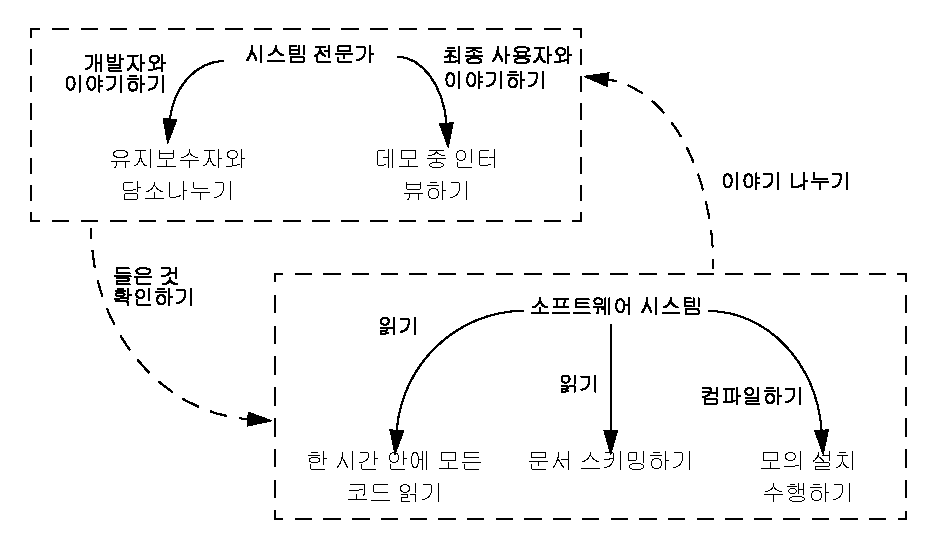
\includegraphics[width=\textwidth]{oldFirstContactMap.pdf}
\caption{시스템에 \charef{첫 번째 접근}{FirstContact}을 진행하는 동안 프로젝트의 \emph{구현가능성(feasbility)}을 평가한다.}
\figlabel{FirstContactMap}
\end{center}
\end{figure}

시스템과 처음 접촉할 때 시간 낭비가 가장 큰 리스크이므로 이러한 패턴은 1주일 정도의 짧은 기간 동안 적용해야 한다. 이번 주가 지나면 주요 이슈를 파악하고 그 지식을 바탕으로 추가 활동을 계획하거나 --- 필요한 경우 --- 프로젝트를 취소해야 한다.

\patref{유지보수자와 담소나누기}{ChatWithTheMaintainers} 및 \patref{데모 중 인터뷰하기}{InterviewDuringDemo} 패턴은 관련된 사람들과 친해지는 데 도움이 될 것이다. 경험상 4일 동안 정보를 수집하고 마지막 날을 사용하여 이 모든 정보를 첫 번째 프로젝트 계획으로 정리하자. 패턴을 적용하는 데 엄격한 순서는 없지만 책에서 제시하는 순서가 일종의 일반적인 순서이다. 그럼에도 불구하고 재차 확인해야 할 필요성 때문에 이러한 패턴의 조각을 조합하는 경우가 종종 있다. 예를 들어 유지보수자(maintainer)와의 두 번째 미팅에서는 보통 \patref{데모 중 인터뷰하기}{InterviewDuringDemo}로 시작하지만 \patref{한 시간 안에 모든 코드 읽기}{ReadAllTheCodeInOneHour}와 \patref{문서 스키밍하기}{SkimTheDocumentation}에서 배운 내용에 대해 질문을 하기도 한다. 또한 인터뷰가 끝나면 소스 코드와 문서를 빠르게 확인하여 말한 내용을 확인한다.

특정 상황에서는 리소스 부족으로 인해 일부 패턴이 적용되지 않는 경우가 있다. 예를 들어, 모든 유지보수자가 퇴사한 경우 \patref{유지보수자와 담소나누기}{ChatWithTheMaintainers}를 사용할 수 없다. 또한 특정 시스템에는 외부 사용자 인터페이스가 없기 때문에 최종 사용자와 \patref{데모 중 인터뷰하기}{InterviewDuringDemo}를 시도하는 것이 무의미할 수도 있다. 이러한 패턴 중 일부는 프로젝트 목표와 무관할 수 있으므로 반드시 문제가 되는 것은 아니다. 하지만 리소스의 부재는 프로젝트에 추가적인 리스크을 초래하므로 첫 번째 프로젝트 계획에 이를 기록해야 한다.

%-----------------------------------------------------------------
\subsection*{다음 단계}

필요한 정보를 확보했다면 이제 첫 번째 프로젝트 계획을 작성할 차례이다.이러한 계획은 프로젝트를 시작할 때 일반적으로 사용하는 계획과 매우 유사하므로 회사에서 사용하는 표준 문서 템플릿을 사용해야 한다. 필요한 경우 최소한 다음 항목이 포함되도록 규칙을 수정하자.

\begin{bulletlist}
  \item \emph{프로젝트 범위.}
프로젝트의 배경, 목표, 목표 달성 여부를 확인하는 데 사용할 기준을 포함하여 프로젝트에 대한 (반 페이지의) 간단한 설명을 준비한다. 계획의 이 부분을 작성하려면 \patpgref{사용자 참여시키기}{InvolveTheUsers} 및 \patpgref{맥심에 동의하기}{AgreeOnMaxims}를 사용한다.

  \item \emph{기회.}
프로젝트 목표를 달성하는 데 기여할 것으로 예상되는 요소를 파악하자. 숙련된 유자보수자와 파워 유저의 가용성(availability), 소스 코드의 가독성(readability) 또는 최신 문서의 존재 여부 등 첫 번째 접촉에서 발견한 항목을 나열하자.

  \item \emph{리스크.}
프로젝트 진행 중에 문제를 일으킬 수 있는 요소를 고려하자. 코드 라이브러리가 누락되었거나 테스트 슈트(test suite)가 없는 등 발견하지 못했거나 품질이 떨어지는 항목을 나열하자. 가능하면 각 리스크에 대한 발생가능성(likelihood)(가능성 없음, 가능성 보통, 가능성 높음)과 영향도(impact)(높음, 보통, 낮음)에 대한 평가를 포함하자. 특히 중요 리스크, 즉 발생가능성이 보통/높고 영향이 보통/높은 리스크 또는 가능성이 높고 영향이 낮은 위험에 대해 특별한 주의를 기울여야 합니다.

  \item \emph{진행/진행 불가 결정.}
어느 시점에서 프로젝트를 계속 진행할지 아니면 취소할지 결정해야 한다. 위의 기회와 리스크을 사용하여 그 결정에 대해 토론하자.

  \item \emph{활동.}
(``진행'' 결정의 경우) 프로젝트 목표를 어떻게 달성할 것인지 설명하면서 향후 기간에 대한 조망(fish-eye view)를 준비하자. 조망도에서는 단기 활동은 상당히 상세하게 설명하고, 이후 활동은 대략적인 개요로 충분하다. 대부분의 경우 단기 활동은 \charef{초기 이해}{InitialUnderstanding}에 설명된 패턴과 일치할 것이다. 이후 활동은 이후 챕터를 확인하자.

활동 목록은 기회를 활용하고 (중요한) 리스크 줄여야 한다. 예를 들어, 최신 문서가 있다는 것을 기회로, 테스트 슈트가 없다는 것을 중대한 리스크로 나열한 경우, 문서를 기반으로 테스트 스위트를 구축하는 활동을 계획해야 한다.

\end{bulletlist}

%=================================================================
%:PATTERN -- Chat with the Maintainers
\pattern{유지보수자와 담소나누기}{ChatWithTheMaintainers}

\intent{시스템 유지보수 담당자와의 토론을 통해 프로젝트의 역사적, 정치적 맥락에 대해 배워보자.}

\subsection*{문제}

리엔지니어링하려는 레거시 시스템의 역사적, 정치적 맥락을 제대로 파악하려면 어떻게 해야 하는가?

\emph{이 문제가 어려운 이유는 다음과 같다.}

\begin{bulletlist}
  \item 문서가 있는 경우 일반적으로 솔루션에 대한 결정은 기록하지만 솔루션에 영향을 준 요소에 대해서는 기록하지 않는다. 따라서 시스템의 역사에서 중요한 사건(즉, 역사적 맥락)은 거의 문서화되지 않는다.

  \item 시스템은 가치가 있지만(그렇지 않다면 시스템을 리엔지니어링할 필요가 없다) 경영진은 통제력을 상실했다(그렇지 않다면 시스템을 리엔지니어링할 필요가 없을 것이다). 소프트웨어 시스템과 관련된 사람 중 적어도 일부가 엉망이므로 레거시 시스템의 정치적 맥락은 본질적으로 문제가 있다.

  \item 시스템과 관련된 사람들이 사용자를 오도할 수 있다. 특히 시스템에서 문제가 있는 부분을 담당하거나 자신의 일자리를 보호하려는 경우 고의적으로 사용자를 속이는 경우가 있다. 대부분의 경우, 특히 수석 개발자가 다른 프로젝트에 참여하고 주니어 직원만 남아 시스템 유지보수를 담당할 때 무지에서 비롯된 오해를 불러일으킬 수 있다.

\end{bulletlist}

\emph{그러나 이 문제를 해결할 수 있는 이유는 다음과 같다.}

\begin{bulletlist}
  \item \emph{유지보수 팀(maintenance team)}과 논의할 수 있다. 그들은 원래 시스템 컨텍스트에 대해 모든 것을 알지 못할 수도 있지만 시스템이 현재 상태가 된 경위에 대해서는 상당 부분 알고 있을 가능성이 높다.
\end{bulletlist}

\subsection*{해결}

시스템 유자보수자와 논의하자. 레거시 시스템에 밀접하게 관여해 온 기술 담당자들은 시스템의 역사와 그 역사에 영향을 미친 사람 관련 문제를 잘 알고 있다.

오해의 소지가 있는 정보를 피하려면 유자보수자를 ``전우(brothers in arms)''로 대하자. 그들이 하는 일에 대해 설명하는 데 시간을 내준다면 그들의 일을 더 쉽게 해줄 수 있는 것(더 많은 보람, 더 많은 인정, --- 그들을 설득할 가능성이 가장 높은 것)을 제공하는 일종의 협상을 시도해 보자. 이렇게 하면 리엔지니어링 프로젝트의 후반 단계에서 필요한 존경심을 얻을 수 있다는 추가적인 이점도 있다.

\subsubsection*{힌트}

다음은 유자보수자와 논의할 때 도움이 될 수 있는 몇 가지 질문이다. 이러한 질문은 (공식 회의록이나 안건이 없는) 비공식 회의 중에 하는 것이 가장 좋지만, 회의가 끝난 후 주요 결론, 가정 및 우려 사항을 기록하기 위해 메모할 준비를 해야 한다.

\begin{bulletlist}
  \item 지난 한 달 동안 가장 쉽게 고칠 수 있었던 버그는 무엇이었나? 그리고 가장 어려웠던 버그는 무엇이었나? 각각을 고치는 데 얼마나 걸렸나? 특정 버그를 고치는 것이 왜 그렇게 쉬웠거나 어려웠나?

이러한 질문은 유지보수 작업에 관심이 있다는 것을 보여주기 때문에 좋은 출발점이 된다. 또한 이러한 질문에 답함으로써 유지보수자는 자신의 뛰어난 능력을 보여줄 수 있는 기회를 얻게 되어 업무에 대한 부담감을 덜 수 있다. 마지막으로, 답변은 나중에 더 높은 수준의 토론에서 사용할 수 있는 \ind{유지보수} 문제에 대한 몇 가지 구체적인 예를 제공한다.

  \item 유지보수 팀은 \ind{버그 리포트}\emph{(bug report)} 및 기능 요청을 어떻게 수집하는가? 어떤 요청을 먼저 처리할지는 누가 결정하는가? 버그 리포팅이나 기능 요청을 관리자에게 배정하는 것은 누가 결정하는가? 이러한 이벤트는 어떤 종류의 데이터베이스에 기록되는가? 버전 또는 구성 관리 시스템(configuration management system)\footnote{소프트웨어의 변경사항을 체계적으로 추적하고 통제하는 시스템으로 형상 관리 시스템이라고도 한다. git도 한 예이다. -옮긴이}이 마련되어 있는가?

이러한 질문은 유지보수 프로세스의 조직과 유지보수 팀의 내부 작업 습관을 이해하는 데 도움이 된다. 정치적 맥락에 관한 한 팀 내 관계(작업 할당)와 최종 사용자와의 관계(버그 리포트 수집)를 평가하는 데 도움이 된다.

  \item 오랫 동안 개발/유지보수 팀의 일원이었던 사람은 누구였는가? 프로젝트에 어떻게 합류/탈퇴했나? 이것이 시스템의 릴리스 기록에 어떤 영향을 미쳤나?

이러한 질문은 레거시 시스템의 역사를 직접적으로 다루는 질문이다. 사람들은 일반적으로 이전 동료에 대해 잘 기억하기 때문에 사람에 대해 물어보는 것이 좋다. 나중에 그들이 어떻게 프로젝트에 합류하거나 떠났는지 물어보면 정치적 맥락도 파악할 수 있다.

  \item 코드는 얼마나 좋은가? 문서는 얼마나 신뢰할 수 있는가?

이 질문은 특히 유지보수 팀 스스로가 시스템 상태를 얼마나 잘 평가할 수 있는지 확인하는 것과 관련이 있다. 물론 나중에 그들의 주장을 직접 확인해야 한다(\patref{한 시간 안에 모든 코드 읽기}{ReadAllTheCodeInOneHour} 및 \patref{문서 스키밍하기}{SkimTheDocumentation} 참조).

  \item 이 리엔지니어링 프로젝트를 시작한 이유는 무엇인가? 이 프로젝트에서 무엇을 기대하는가? 결과를 통해 무엇을 얻을 수 있는가?

리엔지니어링 프로젝트를 통해 유지보수자가 무엇을 얻을 수 있는지 묻는 것은 이후 단계에서 염두에 두어야 할 사항이므로 매우 중요히다. 경영진이 프로젝트에서 기대하는 것과 유지보수자가 기대하는 것의 (때로는 미묘한) 차이점에 귀를 기울이자. 차이점을 파악하면 정치적 맥락을 파악하는 데 도움이 된다.

\end{bulletlist}

\subsection*{트레이드오프}

\subsubsection*{장점}
\begin{bulletlist}
  \item \emph{정보를 효과적으로 얻는다.}
소프트웨어 시스템의 수명 주기에서 중요한 이벤트는 대부분 구두로 전달된다. 유지보수자와 토론하는 것이 이 풍부한 정보 소스를 활용하는 가장 효과적인 방법이다.

  \item \emph{동료와 친해지자.}
관리자와 토론하면 동료에 대해 처음으로 평가할 수 있는 기회를 갖게 됩니다. 따라서 리엔지니어링 프로젝트의 후반 단계에서 필요한 신뢰를 얻을 수 있을 것입니다.

\end{bulletlist}

\subsubsection*{단점}

\begin{bulletlist}
  \item \emph{사례 증거만 제공된다.}
여러분이 얻는 정보는 기껏해야 사례(anecdotal)일 뿐이다. 인간의 뇌는 어떤 사실을 기억하는지에 대해 선택적일 수밖에 없으므로 관리자의 기억이 불충분할 수 있다. 더 나쁜 것은 유지보수자가 시스템의 원래 개발자가 아닌 경우가 많기 때문에 정보가 처음부터 불완전할 수 있다는 것이다. 따라서 다른 방법으로 얻은 정보를 보완해야 한다(예: \patref{문서 스키밍하기}{SkimTheDocumentation}, \patref{데모 중 인터뷰하기}{InterviewDuringDemo}, \patref{한 시간 안에 모든 코드 읽기}{ReadAllTheCodeInOneHour} 및 \patref{모의 설치 하기}{DoAMockInstallation} 참조).

\end{bulletlist}

\subsubsection*{어려움}

\begin{bulletlist}
  \item \emph{사람들은 자신의 일자리를 보호한다.}
일부 유지보수자는 일자리를 잃을까 두려워서 필요한 정보를 제공하지 않을 수도 있다. 리엔지니어링 프로젝트가 그들의 업무를 더 쉽고, 더 보람 있고, 더 가치 있게 만들기 위해 존재한다는 것을 설득하는 것은 여러분의 몫이다. 따라서 유지보수자에게 리엔지니어링 프로젝트에서 무엇을 기대하는지 직접 물어봐야 한다.

  \item \emph{팀이 불안정할 수 있다.}
소프트웨어 유지보수는 일반적으로 2급 업무로 간주되어 주니어 프로그래머에게 맡기는 경우가 많으며 유지보수 팀이 자주 바뀌는 경우가 많다. 이러한 상황에서는 유자보수자가 소프트웨어 시스템의 역사적 진화에 대해 말할 수는 없지만, 그 정치적 맥락에 대해서는 많은 것을 알 수 있다. 실제로 팀의 불안정성은 프로젝트의 위험을 증가시키고 획득한 정보의 신뢰성을 떨어뜨리기 때문에 이러한 불안정성을 인지해야 한다. 따라서 수년 동안 개발/유지보수 팀의 일원이었던 사람이 누구인지 물어봐야 한다.

\end{bulletlist}

\subsection*{예시}

\emph{XDoctor}를 인수하는 동안 회사는 원래 개발 팀을 설득하여 두 소프트웨어 시스템을 하나로 통합하려고 노력해 왔다. 안타깝게도 팀원 중 한 명인 데이브만 남기로 동의하고 나머지 세 명은 다른 회사로 떠났다. 두 제품을 통합하는 방법에 대한 계획을 개발하는 것이 당신의 임무이므로 데이브를 점심 식사에 초대하여 시스템에 대한 비공식적인 대화를 나눈다.

이 대화를 통해 많은 것을 배우게 된다. 좋은 소식은 데이브가 건강 보험과의 거래를 처리하는 인터넷 통신 프로토콜을 구현하는 일을 담당했다는 것이다. 이 기능은 제품에 부족한 핵심 기능 중 하나였기 때문에 팀에 이러한 경험을 추가하게 되어 당신은 기쁠 것이다. 더 좋은 소식은 데이브의 전 동료가 객체 지향 기술에 대한 경험이 많았기 때문에 합리적인 설계와 가독성 높은 소스 코드를 기대할 수 있다는 것이다. 마지막으로 버그 리포트가 거의 제출되지 않았고 대부분의 버그가 빠르게 처리되었다는 이야기도 들었다. 마찬가지로 보류 중인 제품 개선 사항 목록이 존재하며 그 수가 상당히 적다. 따라서 고객들이 제품에 상당히 만족하고 있으며 이 프로젝트가 전략적으로 중요할 것이라고 결론을 내린다.

좋지 않은 소식은 데이브가 주로 동료들에게 무시당하고 나머지 시스템의 설계 활동에서 제외된 하드코어 C 프로그래머라는 것이다. 프로젝트에 남게 된 동기에 대해 물었을 때 그는 원래 인터넷 기술을 실험하는 데 관심이 있어서 합류했지만, 지금까지 해온 저수준 프로토콜 작업이 지루해져서 더 흥미로운 일을 하고 싶다고 말한다. 물론 '더 흥미로운 일'이 무슨 뜻인지 물어보니 그는 객체로 프로그래밍하고 싶다고 대답한다.

토론이 끝난 후 데이브가 작성한 코드의 품질을 평가하기 위해 소스 코드를 확인하기로 마음먹었다. 또한 보류 중인 버그 목록과 개선 요청을 살펴보고 병합해야 할 두 제품의 기능을 비교하고자 한다. 마지막으로 교육 부서에 연락하여 객체 지향 프로그래밍에 대한 강좌가 있는지 알아보는 것도 새 팀원에게 동기를 부여할 수 있는 방법이 될 수 있으므로 고려한다.

\subsection*{근거}

\index{디마르코, 톰}
\begin{quotation}
\noindent
\emph{``우리 업무의 주요 문제는 본질적으로 기술적인 것이 아니라 사회학적 문제이다.''}

\hfill --- 톰 디마르코, \cite{DeMa99a}
\end{quotation}

소프트웨어 프로젝트와 관련된 사회학적 문제가 기술적인 문제보다 훨씬 더 중요하다는 전제를 받아들인다면, 리엔지니어링 프로젝트 참여자들은 최소한 연구 대상 시스템의 정치적 맥락을 알아야 합니다.

\index{콘웨이, 멜빈}
\begin{quotation}
\noindent
\emph{``시스템을 설계하는 조직은 해당 조직의 커뮤니케이션 구조를 복사한 디자인을 만드는 제약을 가진다.''}

\hfill --- Melvin Conway, \cite{Conw68a}
\end{quotation}

\ind{콘웨이의 법칙}\emph{(Conway's law)}은 종종 다음과 같이 의역됩니다: ``컴파일러를 개발하는 그룹이 4개라면, 4패스 컴파일러(4-pass compiler)\footnote{4번의 분리된 단계를 거쳐야만 결과가 나오는 컴파일러-옮긴이}를 얻을 수 있다''

개발팀이 어떤 방식으로 구성되었는지 아는 것이 중요한 이유 중 하나는 이 구조가 소스 코드의 구조를 어느 정도 반영할 가능성이 높기 때문이다.

두 번째 이유는 리엔지니어링 프로젝트 계획을 수립하기 전에 팀원의 역량과 리버스 엔지니어링할 소프트웨어 시스템의 특성을 알아야 하기 때문이다. 유지보수자와의 토론은 이러한 지식을 얻는 방법 중 하나이며, ``시간은 부족하다(time is scarce)''는 원칙을 고려할 때 매우 효율적인 방법이다.

\index{톰셋, 롭}
\begin{quotation}
\noindent
\emph{``유지 보수 관련 사실 \#1. 60년대 후반과 70년대 내내 생산 시스템 지원 및 유지보수는 분명히 2급 업무(second-class work)로 취급되었다.\\.
유지보수 관련 사실 \#2. 1998년에도 생산 시스템 지원 및 유지보수는 계속해서 2급 업무로 취급되었다.''}

\hfill --- 롭 톰셋, \cite{Thom98a}
\end{quotation}

유지보수자와 이야기를 나누다 보면 소프트웨어 유지 관리가 2급 업무로 간주되는 경우가 많다는 사실을 알게 된다. 만약 여러분이 대화하는 유지보수 팀이 그런 경우라면 논의가 심각하게 방해받을 수 있다. 유지보수 팀이 자주 바뀌었기 때문일 수도 있고, 이 경우 유지보수자가 그간의 발전 과정을 잘 모르기 때문일 수도 있다. 또는 논의하는 사람들이 자신의 업무에 대해 매우 보호적인 태도를 취하기 때문에 여러분이 알아야 할 내용을 알려주지 않을 수도 있다. 

\subsection*{알려진 용도}

리엔지니어링 프로젝트를 진행하면서 유지보수 팀과의 회의를 하는 중에 프로젝트의 킥오프(kick-off)하는 습관을 만들었다. 돌이켜보면 이러한 회의가 나머지 프로젝트에 필요한 신뢰를 구축하는 데 얼마나 중요한지 알 수 있었다. 유자보수자는 자신의 직업에 대한 자부심이 강하고 비판에 매우 민감하다는 사실을 뼈저리게 깨달았다. 따라서 킥오프 미팅은 ``유자보수자 중심(maintainer oriented)''으로, 즉 유자보수자가 무엇을 잘하고 무엇을 더 잘하고 싶은지 보여줄 수 있도록 해야 한다는 점을 강조합니다. 초보인 내가 이 멍청한 관리자들에게 제대로 된 일을 하는 방법을 가르쳐주겠다는 태도로 참여하면 거의 틀림없이 재앙을 초래할 것입니다.

\index{루가버, 스펜서}
\index{화이트, 짐}
\begin{quotation}
\noindent
\emph{``\ind{RT-100} ---은 1980년대 후반 타사 소프트웨어 공급업체가 개발하여 1990년에 \ind{노텔(Nortel)}에 인수되었다. 이후 3년 동안 노텔은 이 시스템을 개선하고 유지보수한 후 다른 공급업체에 아웃소싱하여 체계적으로 재작성했다. 이 노력은 실패로 돌아갔고 시스템은 1994년 중반에 다시 노텔로 돌아왔다. 이 무렵에는 원래 설계 팀이 해체되어 흩어져 있었고 제품의 6개 고객 조직은 상당히 불만이 많았다.\\
RT-100은 노텔의 애틀랜타 테크놀로지 파크 연구소에 배정되었다. 그곳에는 ACD 소프트웨어에 대한 경험이 있는 직원이 없었고, 다른 프로젝트의 취소로 인해 직원들의 사기가 상당히 저하되어 있었다.''}

\hfill --- 스펜서 루가버, 짐 화이트, \cite{Ruga98a}
\end{quotation}

위의 인용문은 한 리엔지니어링 프로젝트의 사례를 설명하는 논문에서 인용한 것으로, 리엔지니어링 프로젝트가 시작될 때의 전형적인 절박함을 잘 묘사하고 있다. 하지만 --- 논문 자체에 설명되어 있듯이 --- 역사적, 정치적 맥락에 대한 이러한 초기 평가 덕분에 프로젝트가 성공할 수 있었던 것은 어떤 요소가 이해관계자들을 만족시키고 결과적으로 새로운 리엔지니어링 팀에게 동기를 부여할 수 있는지 잘 알고 있었기 때문이다.

\index{쿡, 스테펀}
\ind{DESEL 프로젝트}(시스템 진화의 용이성을 위한 설계)의 사례 연구 중 하나에서 스테펀 쿡은 도메인의 어떤 측면이 변경될 가능성이 있고 어떤 측면이 안정적으로 유지될 가능성이 있는지 가장 잘 알고 있는 유지보수자와 대화하는 것이 중요하다고 말한다 \cite{Cook01a}. 따라서 유자보수자는 시스템이 어떻게 구축될 수 있었는지에 대한 지식, 즉 거의 문서화되지 않은 지식을 가지고 있다. 그러나 이 논의 과정에서 ``진화를 위한 설계(design for evolution)''라는 사고방식을 강조하여 유자보수자가 자신이 해결해 온 최신의 여러 문제에서 벗어나도록 해야 한다.

\subsection*{관련 패턴}

소프트웨어 개발 팀의 조직 방식을 명시적으로 다루는 몇 가지 패턴 언어가 있다 \cite{Copl95d} \cite{Harri96a} \cite{Tayl00a} \cite{Beed00a}. 앞으로의 엔지니어링 상황을 위한 것이지만, 유지보수자와 논의할 때 상황을 더 빨리 평가하는 데 도움이 될 수 있으므로 이를 숙지하는 것이 좋다.

\subsection*{다음 단계}

토론하는 동안 섣불리 결론을 내리지 않도록 주의해야 한다. 따라서 토론을 통해 알게 된 내용은 다른 출처를 통해 확인해야 한다. 일반적으로 이러한 출처는 시스템을 사용하는 사람들(\patref{데모 중 인터뷰하기}{InterviewDuringDemo}), 문서(\patref{문서 스키밍하기}{SkimTheDocumentation}), 시스템 자체(예: \patref{한 시간 안에 모든 코드 읽기}{ReadAllTheCodeInOneHour}) 등이다. \patref{모의 설치 수행하기}{DoAMockInstallation}).

이 검증을 통해 프로젝트를 완전히 취소할 가능성을 포함하여 레거시 시스템 문제를 해결하기 위한 초기 계획을 세울 수 있는 확실한 근거를 마련할 수 있다. 유자보수자와의 논의는 다양한 방식으로 이 계획에 영향을 미친다. 우선, 유지보수 팀의 협력 의지를 파악할 수 있어 작업 계획에 상당한 영향을 미친다. 둘째, 시스템을 가치 있게 만드는 부분과 대부분의 유지보수 문제를 일으킨 이벤트를 포함하여 시스템의 역사를 알고 있다. 당신 회사의 계획은 가치 있는 부분을 되살리고 이러한 유지보수 문제를 해결하는 것을 목표로 할 것이다. 셋째, 유지보수 팀이 다른 이해관계자들과 어떻게 소통하는지에 대해 알게 되며, 이는 계획이 받아들여지는 데 중요하다.

%=================================================================
%:PATTERN -- Read all the Code in One Hour
\pattern{한 시간 안에 모든 코드 읽기}{ReadAllTheCodeInOneHour}

\intent{간단하지만 집중적인 코드 검토를 통해 소프트웨어 시스템의 상태를 평가한다.}

\subsection*{문제}

소스 코드의 품질에 대한 첫인상을 어떻게 얻을 수 있는가?

\emph{이 문제는 다음과 같은 이유로 어렵다.}

\begin{bulletlist}
  \item 소스 코드의 품질은 시스템의 개발 및 유지보수에 참여한 사람에 따라 상당히 달라질 수 있다.

  \item 시스템 규모가 커서 정확한 평가를 위해 검사해야 할 데이터가 너무 많다.

  \item 소프트웨어 시스템에 익숙하지 않아서 관련성이 있는 것을 필터링하는 방법을 모른다.
\end{bulletlist}

\emph{그러나 이 문제를 해결할 수 있는 이유는 다음과 같다.}

\begin{bulletlist}
  \item 여러분이 구현에 사용 중인 언어에 대한 합리적인 \emph{전문성(expertise)}이 있으므로 프로그래밍 관용구(programming idioms) 및 코드 스멜(code smells)을 인식할 수 있다.

  \item 여러분의 리엔지니어링 프로젝트에 명확한 목표가 있으므로 그 목표를 달성하는 데 필요한 코드 품질을 평가할 수 있습니다.

\end{bulletlist}

\subsection*{해결}

소스 코드를 읽을 수 있는 적당히 짧은 시간(예: 약 1시간)의 학습 시간을 스스로에게 부여하자. 방해받지 않도록 하고(전화기를 뽑고 이메일 연결을 끊고), 코드와 최대한 접촉할 수 있도록 메모를 아껴서 하자. 

이 읽기 세션이 끝나면 다음과 같은 내용을 포함한 간단한 보고서를 작성하자.
\begin{bulletlist}
  \item 리엔지니어링이 실현 가능한지 여부와 그 이유(혹은 안 되는 이유)에 대한 일반적인 평가 항목

  \item 중요해 보이는 엔티티(예: 클래스, 패키지, $\cdots$)

  \item 파악된 의심스러운 코딩 스타일(예: ``\ind{코드 스멜}'' \cite{Fowl99a});

  \item 추가 조사가 필요한 부분(예: 테스트).

\end{bulletlist}

이 보고서는 짧게 작성하고 소스 코드에 언급된 대로 엔티티의 이름을 언급한다.

\subsubsection*{힌트}

``시간은 부족하다(time is scarce)''는 원칙에 따라 약간의 준비가 필요하다. 체크리스트를 작성하면 읽기 세션에서 집중하는 데 도움이 될 수 있다. 이러한 체크리스트는 다양한 출처에서 가져와 작성할 수 있다.

\begin{bulletlist}
  \item 개발 팀에서 품질 보증의 일환으로 \emphind{코드 리뷰}\emph{(code review)}를 사용했을 수 있다. 사용했다면 리뷰에 사용된 체크리스트를 포함해야 한다. 그렇지 않다면 해당 코드의 종류를 검토하는 데 사용되는 일반적인 체크리스트를 사용해 보자.

  \item 일부 개발팀에서는 \emph{코딩 스타일(coding style)}을 적용하기도 하는데, 적용했다면 이를 알아두는 것이 좋다. 특히 명명 규칙(naming convention)은 코드를 빠르게 스캔하는 데 매우 중요하다.

  \item 프로그래머는 \emphind{코딩 이디엄}\emph{(coding idiom)}(예: C++ \cite{Copl92a} \cite{Meye98a} \cite{Meye96a}; Smalltalk \cite{Beck97a})를 사용하여 일반적인 언어 구성을 인식할 수 있다.

  \item 답변을 듣고 싶은 \emph{질문(question)}이 있을 수 있다.
\end{bulletlist}

다음은 추가 검토를 위한 좋은 시작점을 제공하기 때문에 체크리스트에 추가할 수 있는 몇 가지 항목이다.

\begin{bulletlist}
  \item \emph{기능 테스트(functonal test) 및 \ind{단위 테스트}(unit test)}는 소프트웨어 시스템의 기능에 대한 중요한 정보를 전달한다. 이러한 테스트는 시스템이 예상대로 작동하는지 확인하는 데 도움이 되며, 이는 리엔지니어링 중에 매우 중요하다(\charef{테스트라는 생명 보험}{TestsYourLifeInsurance} 참조).

  \item \emph{추상 클래스 및 메서드}는 설계 의도를 드러낸다.

  \item 계층 구조에서 상위 클래스는 종종 도메인 추상화를 정의하고, 하위 클래스는 이에 대한 변형을 도입하도록 돕는다.

  \item \patpgref{싱글톤}{Singleton} 패턴의 발생은 시스템의 전체 실행에 대해 일정한 정보를 나타낼 수 있다.

  \item 놀랍게도 \emph{대형 구조체}는 종종 중요한 기능 덩어리를 지정한다.

  \item \emph{주석(comment)}은 특정 코드의 설계 의도에 대해 많은 것을 알려주지만, 종종 오해의 소지가 있을 수 있다.

\end{bulletlist}


\subsection*{트레이드오프}

\subsubsection*{장점}
\begin{bulletlist}
  \item \emph{효율적으로 시작하자.}
짧은 시간 안에 코드를 읽는 것은 초보자로서 매우 효율적이다. 실제로 시간을 제한하면서도 모든 코드를 살펴보도록 강요하면 두뇌와 코딩 전문 지식을 주로 사용하여 중요해 보이는 부분을 걸러낼 수 있다.

  \item \emph{성실하게 판단하자.}
코드를 직접 읽으면 소프트웨어 시스템에 대한 편견 없는 시각을 갖게 되고, 세부 사항에 대한 감각과 직면하고 있는 문제의 종류를 엿볼 수 있다. 소스 코드는 시스템의 기능을 설명하기 때문에 그 이상도 이하도 아닌 유일한 정확한 정보의 원천이다.

  \item \emph{개발자 어휘를 익히자.}
소프트웨어 시스템 내부에서 사용되는 어휘를 습득하는 것은 시스템을 이해하고 다른 개발자와 소통하는 데 필수적이다. 이 패턴은 이러한 어휘를 습득하는 데 도움이 된다.

\end{bulletlist}

\subsubsection*{단점}
\begin{bulletlist}
  \item \emph{낮은 수준의 추상화만 획득가능하다.}
이 패턴을 통해 솔루션 도메인에 대한 인사이트를 어느 정도 얻을 수 있지만, 이것이 문제 도메인 개념에 어떻게 매핑되는지에 대해서는 거의 알 수 없다. 따라서 더 추상적인 다른 표현으로 얻은 정보를 보완해야 한다(예: \patref{문서 스키밍하기}{SkimTheDocumentation} 및 \patref{데모 중 인터뷰하기}{InterviewDuringDemo}).
\end{bulletlist}

\subsubsection*{어려움}

\begin{bulletlist}
  \item \emph{큰 규모를 다루기 어렵다.}
\emph{모두}를 읽는 방법은 크기가 큰 코드를 다루기 어렵게 하며, 경험상 시간당 10,000줄의 코드가 적당하다. 크고 복잡한 코드를 마주할 때는 짧은 시간(2시간 이내)에 집중적으로 읽는 것이 가장 효과적이므로 더 많은 시간을 할애하여 코드를 읽으려고 하지 않는다. 대신 소스 코드를 분할할 명확한 기준이 있다면 일련의 세션을 나눠서 진행하자. 그렇지 않다면 모든 코드를 살펴보고 다른 부분보다 더 중요해 보이는 부분을 표시한 다음 \patref {유지보수자와 담소나누기}{ChatWithTheMaintainers}에 따라 다른 세션에서 읽으면 된다.

그러나 ``시간은 부족하다(Time is Scarce)''는 원칙을 고려할 때 간결하게 작성해야 한다. 따라서 크고 복잡한 코드를 다룰 때는 세부 사항에 너무 신경 쓰지 말고 리엔지니어링 적합성에 대한 초기 평가라는 코드 읽기의 목표를 상기하자.

  \item \emph{주석이 오해를 불러일으킬 수 있다.}
코드의 주석에 주의를 기울이자. 코멘트는 소프트웨어의 기능을 이해하는 데 도움이 될 수 있다. 하지만 다른 종류의 문서와 마찬가지로 주석도 오래되었거나 더 이상 사용되지 않거나 단순히 잘못된 것일 수 있다. 따라서 주석을 찾을 때는 체크리스트에 해당 주석이 도움이 되는지, 오래되었는지 여부를 표시하자.
\end{bulletlist}

\subsection*{예시}

데이브(원래 개발팀에서 유일하게 남은 사람으로 저수준 C 코드를 담당했던 사람)와의 토론에서, 여러분은 그들의 시스템이 주로 Java로 작성되었고 일부 저수준 부분은 C로, 데이터베이스 쿼리는 SQL로 작성되었다는 것을 기억할 것이다. 이 모든 언어에 대한 경험이 있으므로 코드를 읽을 수 있다.

먼저 체크리스트를 작성하고 일반적인 항목(코딩 스타일, 테스트, 추상 클래스 및 메서드, 계층 구조에서 상위 클래스, $\cdots$) 외에 해결하고 싶은 몇 가지 질문에 관한 몇 가지 항목을 추가한다. 그 중 하나는 ``C 코드의 가독성(readability of the C-code)''인데, 새 팀원인 데이브의 코딩 스타일을 확인하고 싶기 때문이다. 두 번째는 ``데이터베이스 스키마의 품질(quality of the database schema)''인데, 조만간 두 시스템의 데이터를 통합해야 한다는 것을 알고 있기 때문이다. 세 번째는 ``통화 처리(handling of currencies)''이다. 스위스가 유로 지역에 가입하고 6개월 이내에 모든 금융 데이터를 이 새로운 통화로 변환해야 하기 때문이다.

C 코드를 읽다 보면 이 부분이 상당히 난해하다는 것을 알 수 있다(수수께끼 같은 약어로 된 짧은 식별자, 긴 다중 출구 루프, $\cdots$). 그럼에도 불구하고 인터넷 프로토콜을 처리하는 모듈에는 단위 테스트가 있으므로 시스템에 통합할 가능성에 대해 더 확신을 가질 수 있다.

Java 코드는 한 시간에 50.000줄의 코드를 읽을 수 없다는 규모의 문제가 있다. 따라서 무작위로 몇 개의 파일을 선택하면 대부분의 클래스 이름에 \ct{UI} 또는 \ct{DB}라는 두 글자 접두사가 붙는 것을 발견할 수 있다. 2 계층 아키텍처(2-tiered architecture)(데이터베이스 계층과 사용자 인터페이스 계층)를 나타내는 명명 규칙을 의심하고 이를 자세히 조사하기 위해 메모를 작성한다. 또한 다양한 클래스 및 속성 이름이 의료 도메인에 의미 있는 것으로 인식한다(예: 이름, 주소, 건강 보험, $\cdots$ 속성을 가진 클래스 \ct{DBPatient}). 심지어 \ct{DBCurrency} 클래스를 인식하므로 개발자가 필요한 예방 조치를 취했기 때문에 유로로 전환해도 큰 문제가 발생하지 않을 것이라고 가정한다. 대부분의 클래스와 메서드에는 \ind{Javadoc} 규칙을 따르는 주석이 있으므로 적어도 일부 문서는 최신 상태일 것으로 예상한다. 마지막으로, 화면에 표시되는 다양한 문자열을 포함하는 대형 싱글톤 객체를 식별하여 시스템을 지역화할 수 있을 것이라는 결론을 내린다.

이 모든 것이 다소 희망적으로 보이지만 실망스러운 부분도 많이 있다. 가장 비관적인 이유는 매개변수 목록이 많고 조건문이 복잡한 긴 메서드가 많다는 점이다. 이들 중 상당수는 UI 로직(버튼과 메뉴 항목의 활성화/비활성화)과 비즈니스 로직(데이터베이스 레코드 업데이트)이 혼합되어 있는 것 같다. 한 가지(가격 계산)가 특히 복잡해 보이므로 이를 더 조사하기 위해 메모를 작성한다.

데이터베이스와 관련해서는 의료 서비스 도메인의 맥락에서 의미 있는 다양한 테이블 이름과 열 이름을 다시 인식한다. 언뜻 보기에는 스키마가 정규화된 것처럼 보이므로 여기에서도 리버스 엔지니어링이 횩허거 있을 것으로 보인다. 이 데이터베이스는 또한 일부 저장 프로시저를 사용하므로 추가 조사가 필요하다.

읽기 세션이 끝나면 다음 노트에 결론을 요약한다.

\begin{bulletlist}
  \item 인터넷 프로토콜 통합이 가능함: 단위 테스트와 담당 프로그래머가 있다.

  \item 명명 규칙에 따라 2계층 아키텍처가 의심됨: 비즈니스 로직은 어떤가? --- UI와 혼합되어 있는가? (추가 확인 필요!)

  \item 의미 있는 식별자가 포함되어 있는 읽을 수 있는 코드: 리버스 엔지니어링의 효과가 기대된다.

  \item 통화 개체 존재: 유로 변환이 가능해 보인다(추가 조사!).

  \item 사용된 자바독(Javadoc) 규칙 사용: 문서 확인이 필요하다.

  \item 가격 계산이 복잡해 보임: 그 이유는 무엇인가?

  \item 데이터베이스 스키마가 유용해 보임: 저장 절차는 추가 조사가 필요합니다.

\end{bulletlist}

\subsection*{근거}

코드 리뷰(coder review)는 동료가 작성한 프로그램에서 문제를 찾는 데 매우 효과적인 수단으로 널리 인정받고 있다 \cite{Gilb93a} \cite{Glass97a}. 이러한 검토를 비용 효율적으로 수행하기 위해서는 두 가지 중요한 전제 조건이 충족되어야 합니다: (a) 검토자가 관련 질문에 집중할 수 있도록 \emph{체크리스트(checklist)}를 준비해야 하고, (b) 리뷰어는 장시간(최대 2시간) 집중할 수 없으므로 리뷰 세션은 \emph{짧게} 유지해야 한다.

\index{코니그스버그, 앨런}
\begin{quotation}
\noindent
\emph{나는 속독 강좌를 들었고 '전쟁과 평화'를 20분 만에 읽었다. 러시아에 관한 책이다.}

\hfill --- 우디 앨런
\end{quotation}

기존의 코드 리뷰와 소프트웨어 시스템을 처음 접할 때 수행하는 코드 리뷰에는 중요한 차이점이 있다. 전자는 일반적으로 오류를 감지하기 위한 것이고, 후자는 첫인상을 얻기 위한 것이다. 이 차이는 세부 사항에 덜 신경을 써야 하므로 더 많은 코드를 읽을 수 있다는 것을 의미한다. 코드 리뷰에 대한 일반적인 가이드라인에서는 시간당 약 150개의 문을 검토할 수 있다고 명시하고 있다 \cite{Barn94a}. 그러나 첫 번째 접촉에서는 이러한 상세한 분석이 필요하지 않으므로 검토할 코드의 양을 늘릴 수 있다. 심각한 경험적 조사를 수행하지는 않았지만 경험상 시간당 10,000줄의 코드가 적당해 보인다.

\subsection*{알려진 용도}

\index{벡, 켄트}
이 패턴은 켄트 벡이 제안한 것으로, 그는 기존 시스템에서 컨설턴트 업무를 시작할 때 항상 적용하는 기법 중 하나라고 말했다. 롭슨은 코드 읽기를 ``시스템에 대한 지식을 얻는 가장 조잡한 방법(crudest method)''으로 보고하며, 기존 프로그램을 이해하는 데 가장 일반적으로 사용되는 방법이라고 인정한다{Robs91a}. 일부 사례 연구 보고서에서도 소스 코드 읽기가 리엔지니어링 프로젝트를 시작하는 방법 중 하나라고 언급하고 있다 \cite{Bray95a} \cite{Jack00a}.

이 패턴을 작성하는 동안 우리 팀원 중 한 명이 이 패턴을 적용하여 \ind{리팩토링 브라우저}(Refactoring Browser)를 리버스 엔지니어링했다. \cite{Robe97a}. 그 사람은 \ind{Smalltalk}에 익숙하지 않았지만 클래스 인터페이스를 검사하는 것만으로도 시스템 구조에 대한 느낌을 얻을 수 있었다. 또한 특수 계층 구조 브라우저는 주요 클래스 중 일부를 식별하는 데 도움이 되었고 주석은 코드의 어떤 부분을 수행해야 하는지에 대한 유용한 힌트를 제공했다. 패턴을 적용하는 데는 1시간이 조금 넘게 걸렸는데, 비교적 작은 시스템과 Smalltalk에 익숙하지 않아서 진행 속도가 느려 보였기 때문에 이 정도면 충분해 보였다.

이 패턴의 특히 흥미로운 사례는 \ind{FAMOOS} 프로젝트가 끝날 무렵에 발생했다. 일주일 동안 이질적인 리버스 엔지니어들로 구성된 팀이 일종의 리버스 엔지니어링 경연 대회에 참가하기 위해 현장 방문을 떠났다. 4일 동안 주어진 리버스 엔지니어링 도구를 사용하여 특정 \ind{C++} 시스템에 대해 최대한 많은 것을 배우는 것이 과제였다. 그런 다음 5일째에는 원래 개발자에게 결과를 보고하여 검증을 받는 것이었다. 팀원 중 한 명이 과제를 너무 일찍 끝내고 \patref{한 시간 안에 모든 코드 읽기}{ReadAllTheCodeInOneHour}에 도전하는 기회를 가졌다. 이 한 사람은 모든 토론에 참여할 수 있고 개발자의 의견 중 일부를 설명할 수 있을 정도로 시스템에 대해 훨씬 더 잘 파악하고 있었습니다.

\subsection*{다음 단계}

\patref{한 시간 안에 모든 코드 읽기}{ReadAllTheCodeInOneHour}를 완료한 후에는 리엔지니어링에 적합한지 평가하기 위해 \patref{모의 설치 수행하기}{DoAMockInstallation}을 수행해야 한다. 또한 \patref{문서 스키밍하기}{SkimTheDocumentation}를 수행하여 결과를 보완하고, 시스템을 일관성 있게 파악할 수 있는 기회를 극대화하기 위해 \patref{데모 중 인터뷰하기}{InterviewDuringDemo}를 수행하면 된다. 실제로 리엔지니어링 프로젝트를 어떻게 진행할지 결정하기 전에 \patref{유지보수자와 담소나누기}{ChatWithTheMaintainers}를 한 번 더 수행하는 것이 좋다.

시스템과의 첫 접촉이 끝나면 프로젝트를 어떻게 진행할지(또는 취소할지) 결정해야 한다. 코드를 읽으면 다양한 방식으로 이 결정에 영향을 미친다. 우선, 코드의 품질(예: 코딩 이디엄 및 의심스러운 코딩 스타일의 존재 여부)을 평가하여 프로젝트 리엔지니어링의 타당성을 평가했다. 둘째, 추가 탐색을 위한 좋은 출발점이 될 수 있는 몇 가지 중요한 엔티티를 식별했다. 

중요한 엔티티(예: 클래스, 패키지, \patref{한 시간 안에 모든 코드 읽기}{ReadAllTheCodeInOneHour}의 결과인 클래스, 패키지, $\cdots$) 목록을 사용하여 \patpgref{퍼시스턴트 데이터 분석하기}{AnalyzeThePersistentData} 및 \patpgref{예외적인 엔티티 연구하기}{StudyTheExceptionalEntities}를 시작할 수 있다. 이렇게 하면 소스 코드, 특히 문제 도메인을 나타내는 방식에 대해 구체적으로 이해할 수 있다.

%=================================================================
%:PATTERN -- Skim the Documentation
\pattern{문서 스키밍하기}{SkimTheDocumentation}

\intent{제한된 시간 내에 \ind{문서}(documentation)를 읽고 관련성을 평가한다.}

\subsection*{문제}

문서에서 도움이 될 수 있는 부분을 어떻게 식별할 수 있는가?

\emph{이 문제는 다음과 같은 이유로 어렵다.}

\begin{bulletlist}
  \item 문서가 있는 경우 개발팀이나 최종 사용자를 위한 것이므로 일반적으로 리엔지니어링 목적과 즉각적인 관련이 없다. 더 좋지 않은 것은 일반적으로 현재 상황과 관련하여 최신 정보가 아니므로 오해의 소지가 있는 정보가 포함되어 있을 수 있다는 것이다.

  \item 리엔지니어링 프로젝트가 어떻게 진행될지 아직 알 수 없으므로 문서의 어느 부분이 관련성이 있는지 알 수 없다.
\end{bulletlist}


\emph{그러나 이 문제를 해결할 수 있는 이유는 다음과 같다.}

\begin{bulletlist}
  \item 어떤 형태의 \emph{문서(documentation)}를 사용할 수 있으므로 적어도 시스템과 관련된 사람을 돕기 위한 설명이 있다.

  \item 여러분의 리엔지니어링 프로젝트에는 \emph{명확한 목표(clear goal)}가 있으므로 문서에서 가치 있는 부분과 쓸모없는 부분을 선택할 수 있다.

\end{bulletlist}

\subsection*{해결}

리엔지니어링 프로젝트에 흥미로워 보이는 시스템 측면을 요약한 목록을 준비하자. 그런 다음, 이 목록을 문서와 대조하면서 문서가 얼마나 최신 상태인지 대략적으로 평가하자. 마지막으로 다음과 같이 간단한 보고서로 결과를 요약하자.

\begin{bulletlist}
  \item 시스템 문서가 유용한지 여부와 그 이유 (혹은 그렇지 않은 이유)에 대한 일반적인 평가를 적는다.

  \item 문서에서 유용하다고 생각되는 부분의 목록과 그 이유(예: 요구 사항 사양, 원하는 기능, 중요한 제약 조건, 설계 다이어그램, 사용자 및 운영자 설명서)를 작성한다.

  \item 각 부분에 대해 설명이 얼마나 최신 상태인지에 대한 인상을 작성한다.
\end{bulletlist}

\subsubsection*{힌트}

리엔지니어링 프로젝트의 목표와 사용 중인 문서의 종류에 따라 주요 관심사에 맞게 읽기 프로세스를 조정할 수 있다. 예를 들어 원래 시스템 요구 사항에 대한 인사이트를 얻고 싶다면 시스템 사양을 살펴보고, 실제로 구현된 기능에 대한 지식은 최종 사용자 설명서나 튜토리얼 노트에서 수집해야 한다. 여유가 있다면 설계 문서(예: 클래스 다이어그램, 데이터베이스 스키마, $\cdots$)를 이해하려고 너무 많은 시간을 소비하지 말고, 리엔지니어링의 후반 단계에서 큰 도움이 될 수 있으므로 이러한 문서의 존재 여부와 신뢰성을 기록해 두자. 

실제 시스템과 관련하여 문서가 오래되지는 않았는지 확인하자. 항상 시스템 납품 날짜와 버전 날짜를 비교하고 신뢰할 수 없는 것으로 의심되는 부분을 기록해 두자. 

시간이 제한되어 있다는 사실 때문에 가장 유용한 정보를 추출할 수 있는 방법을 생각해야 한다. 다음은 주의해야 할 사항에 대한 몇 가지 힌트이다.

\begin{bulletlist}
  \item \emph{목차(table of contents)}는 구조와 제시된 정보에 대한 간략한 개요를 제공한다.

  \item \emph{버전 정보 및 날짜(Version numbers and dates)}는 문서의 해당 부분이 얼마나 최신 상태인지 알려준다.

  \item \emph{그림(figure)}은 정보를 전달하기 위한 좋은 수단이다. 그림 목록이 있는 경우 문서의 특정 부분에 대한 빠른 액세스 경로를 제공할 수 있다.

  \item \emph{화면 덤프(screen-dump), 샘플 출력물(print-out), 샘플 리포트(report), 명령어 설명(command description)}은 시스템에서 제공하는 기능에 대해 많은 것을 알려준다.

  \item \emph{정식 사양(formal specifications)}(예: 상태 차트(state-chart))이 있는 경우 일반적으로 중요한 기능에 해당한다.

  \item \emph{색인(index)}가 있는 경우에는 작성자가 중요하다고 생각하는 용어가 포함되어 있습니다.
\end{bulletlist}

\subsection*{트레이드오프}

\subsubsection*{장점}

\begin{bulletlist}
  \item \emph{높은 추상화 수준을 제공한다.}
문서는 사람이 읽어야 하므로 일정 수준의 추상화가 필요하다. 이 추상화 수준이 리엔지니어링 프로젝트에 충분히 높지 않을 수도 있지만 적어도 몇 가지 디코딩 단계를 건너뛸 수 있다.

  \item \emph{관련 부분에 집중한.}
흥미로워 보이는 부분의 목록을 미리 준비하면 읽기 세션이 목표 지향적이 되어 가치 있는 것을 찾을 확률이 높아진다. 또한 설명이 얼마나 최신인지 빠르게 평가할 수 있어 관련 없는 부분에 시간을 낭비하지 않아도 된다.
\end{bulletlist}

\subsubsection*{단점}

\begin{bulletlist}
  \item \emph{중요한 사실 누락한다.}
개요 모드에서 빠르게 읽으면 문서에 기록된 중요한 사실을 놓칠 수 있다. 하지만 찾고자 하는 내용을 목록으로 작성하면 이러한 효과를 어느 정도 줄일 수 있다.

  \item \emph{관련 없는 정보만 찾을 수 있다.}
문서의 어느 부분도 리엔지니어링 프로젝트와 관련이 없는 것처럼 보일 가능성이 적다. 그런 상황에서도 이제 문서에 대해 걱정하지 않아도 되니 읽는 데 들인 시간은 가치가 있다.

\end{bulletlist}

\subsubsection*{어려움}

\begin{bulletlist}
  \item \emph{다른 청중을 대상으로 한다.}
문서는 제작 비용이 많이 들기 때문에 최종 사용자(예: 사용자 매뉴얼) 또는 개발팀(예: 디자인)을 위해 작성된다. 또한 문서를 유지 관리하는 데도 많은 비용이 들기 때문에 시스템의 안정적인 부분만 문서화한다. 따라서 찾은 정보는 직접적인 관련이 없을 수 있으므로 신중한 해석이 필요하다.

  \item \emph{문서에 불일치가 있다.}
문서는 실제 상황과 관련하여 거의 항상 최신 정보가 아니다. 리엔지니어링 프로젝트의 초기 단계에서는 이러한 불일치를 인식할 수 있는 지식이 부족하기 때문에 이는 매우 위험하다. 따라서 문서에만 의존하여 중요한 결정을 내리지 말고, 먼저 다른 방법으로 결과를 확인하기 바란다, \patref{한 시간 안에 모든 코드 읽기}{ReadAllTheCodeInOneHour} 및 \patref{데모 중 인터뷰하기}{InterviewDuringDemo}).
\end{bulletlist}

\subsection*{예시}

데이브와의 비공식적인 대화와 코드 읽기 세션이 끝나면 시스템의 흥미로운 측면이 무엇인지 대략적으로 파악할 수 있다. 관련 정보가 포함되어 있는지 확인하기 위해 문서를 훑어보기로 결정한다.

읽고 싶은 측면의 목록을 작성하여 스스로 준비한다. 디자인 다이어그램, 클래스 인터페이스 설명(자바독?), 데이터베이스 스키마와 같은 당연한 항목 외에도 유로(사용자 설명서에 유로 변환에 대한 내용이 있는가?), 인터넷 프로토콜 사양 등이 목록에 포함되어 있다.

다음으로 데이브에게 가서 소프트웨어 시스템과 관련된 모든 문서를 요청한다. 데이브는 작은 미소를 지으며 여러분을 바라본다. ``정말 다 읽어보실 건 아니죠?'' ``꼭 그렇지는 않아요.'' ``하지만 적어도 이걸로 뭔가 할 수 있는지는 알고 싶어요.''라고 말한다. 데이브가 아까 준 상자를 살펴보고 종이로 가득 찬 폴더 3개 --- 설계 문서 ---와 소책자 1개 --- 사용 설명서를 건네준다.

사용 설명서부터 시작해서 --- 빙고: 색인에서 유로에 대한 항목을 발견한다. 해당 페이지를 넘기면 유로가 실제로 약 5페이지로 구성된 하나의 챕터라는 것을 알 수 있으므로 해당 페이지 번호를 표시하여 추가 학습을 진행한다. 다음으로 목차를 훑어보면 '프랑스어/독일어로 전환하기'라는 제목이 있다. 이 페이지를 읽으면 소프트웨어 현지화가 문서화된 기능이라는 것을 알 수 있다. 현지화는 체크리스트에 없었지만 여전히 중요하므로 기꺼이 이에 대한 메모를 추가한다. 이 모든 것이 상당히 유망해 보이므로 사용자 설명서의 릴리스 날짜를 확인하면 꽤 최근의 것임을 알 수 있다. 정말 좋은 시작이다!

디자인 문서의 첫 번째 폴더('클래스라는 제목의 폴더)를 열면 예상했던 것과 거의 비슷하게 Javadoc에서 생성된 클래스 인터페이스의 인쇄물을 찾을 수 있다. 종이로 읽는 것은 그다지 흥미롭지 않지만 어쨌든 페이지를 계속 훑어보게 된다. 첫인상은 각 클래스와 메서드와 함께 제공되는 실제 설명이 상당히 얕다는 것이다. 무작위로 세 페이지를 더 자세히 살펴보면 이러한 인상은 더욱 확고해진다. 다음으로 인터넷 프로토콜을 구현하는 C 코드와 인터페이스하는 클래스에 대한 설명을 찾아보면 빈 설명도 발견할 수 있다. 문서의 릴리스 날짜를 리트머스 테스트한 결과 이 문서가 상당히 오래되었다는 것을 알았으므로 온라인 문서를 확인하기 위해 메모를 작성한다.

두 번째 폴더에는 데이터베이스 스키마에 대한 생성된 설명이 들어 있는데, 각 테이블에 대해 각 열의 목적이 무엇인지 설명한다. 자바독 클래스 인터페이스 설명과 마찬가지로 문서 자체는 내용이 적어도 데이터베이스의 각 레코드가 무엇을 나타내야 하는지를 찾을 수 있는 방법이 있다. 여기에서도 문서 릴리스 날짜가 확인하니 동일한 문서의 온라인 버전을 확인하는 것이 필요하다는 것도 알 수 있다.

언뜻 보기에 세 번째 폴더에는 프로젝트와 막연하게 관련만 있어 보이는 다양한 잡다한 문서 사본이 들어 있는 것처럼 보인다. 첫 번째 문서는 의약품 가격 목록이고, 다음 열 개는 의료법에서 발췌한 것이다. 하지만 계속해서 페이지를 넘기다 보면 건강보험과 통신하는 데 사용되는 인터넷 프로토콜을 설명하는 것으로 보이는 유한 상태 다이어그램(finite state diagram)을 발견하게 된다. 분명히 이 문서는 기술 사양의 일부 페이지를 복사한 것이지만 안타깝게도 원본에 대한 참조는 포함되어 있지 않다. 이 문서의 릴리스 날짜도 누락되어 있어 이 사양이 오래된 것인지 확인할 수 있는 방법이 없다.

다음 보고서를 작성하고 읽기 세션을 마무리한다.

\begin{bulletlist}
  \item 사용자 설명서가 명확하고 최신 상태임: 기능에 대한 블랙박스 타입의 설명을 위한 좋은 참고처이다.

  \item 유로 화폐 관련 정보가 제공됨(513-518쪽): 현지화도 제공된다(723-725쪽).

  \item 클래스 인터페이스 설명이 생성되어 있음: 정보가 적지만 온라인에서 확인 가능하다.

  \item 데이터베이스 스키마에 대한 문서가 생성됨: 간략하지만 온라인에서 확인 가능하다.

  \item 인터넷 프로토콜에 대한 유한 상태 머신: 상태 의심스럽다. 데이브에게 에게 확인하도록 한다.

  \item 기타 문서(가격표, 지침 전단지, $\cdots$)가 들어 있는 폴더 1개
\end{bulletlist}

\subsection*{근거}

\index{프레스맨, 로저}
\begin{quotation}
\noindent
\emph{``소프트웨어 개발 조직에서 전체 소프트웨어 개발 노력의 20\~30\%를 문서화에 사용하는 것은 드문 일이 아니다.''}

\hfill --- 로저 프레스맨, \cite{Pres94a} 
\end{quotation}

소스코드와 달리 문서는 소프트웨어 시스템을 인간에게 적합한 추상화 수준에서 설명하기 위한 것이다. 따라서 문서에는 분명히 정보 ``덩어리(nugget)''가 포함될 것이며, 문제는 관련 정보를 찾는 방법이다. 거의 모든 리엔지니어링 프로젝트에 존재하는 두 가지 일반적인 상황 때문에 관련 정보를 찾는 것이 어렵다.

\begin{quotation}
\noindent
\emph{``모든 사례 연구에서 문서가 존재하지 않거나 불만족스럽거나 일관성이 없다는 문제에 직면한다.-''}

\noindent
--- ESEC/FSE 1997 Workshop on Object-Oriented \\
Re-engineering, \cite{Deme97a}
\end{quotation}

우선, 문서가 실제 상황과 일치하지 않을 가능성이 높다. ind{FAMOOS} 프로젝트에서 조사한 5개의 사례 연구에서 모든 관리자가 불만을 제기한 유일한 문제는 '불충분한 문서화'였다. 그럼에도 불구하고 오래된 정보라도 적어도 과거에 시스템이 어떻게 작동해야 했는지 알려주기 때문에 유용할 수 있다. 오늘날 어떻게 사용되는지 유추할 수 있는 좋은 출발점이다.

\index{웡, 케니}
\begin{quotation}
\noindent
\emph{``이러한 시스템에 대해 존재하는 문서는 일반적으로 전체 아키텍처가 아닌 개별적인 부분에 대해 설명한다. 게다가 문서는 시스템 전체와 여러 미디어에 흩어져 있는 경우가 많다.''}

\hfill 케니 웡, \etal, \cite{Wong95a}
\end{quotation}

둘째, 문서는 일반적으로 포워드 엔지니어링 컨텍스트에서 생성되므로 리엔지니어링 목적이 아니다. 예를 들어, 생성된 설계 문서(예: 데이터베이스 스키마, 자바독)는 일반적으로 상당히 최신이지만 너무 세분화되어 있어 리엔지니어링 프로젝트의 초기 단계에서는 유용하지 않다. 사용 설명서는 소프트웨어 시스템에 대한 블랙박스 타입의 설명이므로 그 안에 무엇이 들어 있는지에 대한 청사진 역할을 할 수 없다. 여기에서도 설명서를 실제로 관심 있는 부분을 유추할 수 있는 좋은 출발점으로 삼아야 한다.

\subsection*{알려진 용도}

피엘드슈타트와 햄렌의 연구에 따르면 '유지보수 프로그래머는 기능을 개선할 때 문서를 공부하는 시간보다 원래 프로그램을 공부하는 시간이 약 3.5배 더 길지만, 개선 기능을 구현하는 데 소요되는 시간은 그만큼 더 길다'고 합니다. \cite{Corb89a}, \cite{Fjel79a}. 이 등식은 문서 연구의 상대적 중요성에 대한 설명으로 받아 들일 수 있다.

\index{잭슨, 다니엘}
\index{채핀, 존}
\begin{quotation}
\noindent
\emph{``사례 연구는 CTAS의 기존 설계 전반과 특히 CM을 이해하려는 노력에서 시작되었다. --- CTAS에 대한 문서에는 동기 부여 및 아키텍처 개요, 소프트웨어 구조, 사용자 설명서, 기본 알고리즘에 대한 연구 논문이 포함되어 있다. 그러나 시스템이 무엇을 계산하는지 또는 환경에 대해 어떤 가정을 하는지에 대해 개괄적으로 설명하는 문서는 없는 것으로 보인다. 또한 CTAS 구성 요소 간의 관계(통신 방식, 제공하는 서비스 등)를 설명하는 설계 문서도 없다. 우리는 코드에서 이러한 정보를 유추할 수밖에 없었는데, 이는 많은 상업 개발 노력에 공통적으로 나타나는 문제이다.''}

\hfill --- 다니엘 잭슨, 존 채핀, \cite{Jack00a}
\end{quotation}

위의 인용문은 문서를 공부할 필요가 있다는 것을 잘 요약하고 있지만, 문서가 알아야 할 모든 것을 여러분에게 알려주지는 않는다. 그들이 언급한 사례 연구는 항공 교통 관제 시스템(CTAS)에 관한 것으로, 약 80개의 KLOC C++ 코드로 구성된 핵심 구성 요소 \emph{Communications\-Manager}(CM)를 리버스 엔지니어링한 것이다.

다음 일화는 문서가 어떻게 오해를 불러일으킬 수 있는지를 보여준다. ind{FAMOOS} 사례 연구 중 하나에서 약 12개의 하위 시스템을 연결하는 분산 시스템을 약 100개의 하위 시스템을 연결하도록 확장할 수 있는지 평가해 달라는 요청을 받았다. 이 평가에서 우리는 모든 TCP/IP 연결을 유지 관리하는 클래스를 연구했는데, 이 클래스에서는 모든 열린 연결이 일종의 룩업 테이블에서 어떻게 유지되는지 설명하는 코멘트가 있었다. 코드에서 룩업 테이블을 찾았지만, 그 작동 방식에 대한 설명을 테이블을 조작하는 연산에 매핑할 수는 없었다. 반나절 동안 고민하다가 포기하고 관리자에게 물어보기로 했다. 그의 대답은 ``아, 하지만 이 클래스 주석은 더 이상 사용되지 않아요. 이제야 말씀하시니 그 클래스를 다시 디자인할 때 삭제했어야 했는데요."라는 답변이었다.

\subsection*{다음 단계}

특정 결과를 확인하기 위해 \patref{한 시간 안에 모든 코드 읽기}{ReadAllTheCodeInOneHour} 바로 뒤에 \patref{문서 스키밍하기}{SkimTheDocumentation}을 추가할 수 있습니다. 또한 \patref{유지보수자와 대화나누기}{ChatWithTheMaintainers} 및 \patref{데모 중 인터뷰하기}{InterviewDuringDemo}를 통해 특정 의혹을 확인하는 것도 좋다.

시스템과의 첫 접촉이 끝나면 프로젝트를 어떻게 진행할지 (또는 취소할지) 결정해야 한다. 관련 문서를 발견하면 적어도 이 정보를 재현할 필요는 없다는 것을 알 수 있다. 더 좋은 점은 관련성이 있지만 부정확해 보이는 문서의 경우 추가 탐색을 위한 좋은 출발점이 있다는 것이다(예: \patpgref{퍼시스턴트 데이터 분석하기}{AnalyzeThePersistentData} 및 \patpgref{디자인에 대해 추측하기}{SpeculateAboutDesign}).

%=================================================================
%:PATTERN -- Interview During Demo
\pattern{데모 중 인터뷰하기}{InterviewDuringDemo}

\intent{데모를 보고 데모를 제공하는 사람과 인터뷰하여 소프트웨어 시스템의 기능에 대한 첫인상을 구한다.}

\subsection*{문제}

소프트웨어 시스템의 일반적인 사용 시나리오와 주요 기능에 대한 아이디어를 어떻게 얻을 수 있는가?

\emph{이 문제는 다음과 같은 이유로 어렵다.}

\begin{bulletlist}
  \item 일반적인 사용 시나리오는 사용자 유형에 따라 매우 다양하다.

  \item 사용자에게 물어보면 무엇이 잘못되었는지 불평하는 경향이 있는 반면, 리버스 엔지니어링의 경우 주로 무엇이 가치 있는지에 관심이 있다.

  \item 시스템 규모가 커서 정확한 평가를 위해 검사해야 할 데이터가 너무 많다.

  \item 소프트웨어 시스템에 익숙하지 않아서 관련성이 있는 것을 필터링하는 방법을 모른다.

\emph{하지만 다음과 같은 이유로 이 문제를 해결할 수 있다.}

  \item 작동 중인 시스템과 소프트웨어 시스템 사용 방법을 보여줄 수 있는 사용자가 있다는 점을 활용할 수 있다.
\end{bulletlist}

\subsection*{해결}

데모를 보고 시연하는 사람을 인터뷰하여 작동 중인 시스템을 관찰한다. 인터뷰 부분은 적어도 데모만큼이나 유익하다는 점에 유의하자. 

이 데모가 끝나면 같은 정도의 시간을 할애하여 발견한 내용을 포함한 보고서를 작성하자.

\begin{bulletlist}
  \item 몇 가지 일반적인 사용 시나리오.

  \item 시스템에서 제공하는 주요 기능 및 그 기능에 대한 평가.

  \item 시스템 컴포넌트와 컴포넌트의 책임. 

  \item 시스템 사용과 관련된 숨겨진 이야기를 보여주는 기이한 사례.
\end{bulletlist}

\subsubsection*{힌트}

데모를 제공하는 사용자는 이 패턴의 결과에 결정적인 역할을 하므로 사람을 선택할 때 주의하자. 따라서 데모를 제공하는 사람을 여러 번 바꿔서 데모를 여러 번 수행하자. 이렇게 하면 사람들이 중요하다고 생각하는 요소의 차이를 확인할 수 있고 소프트웨어 시스템의 가치에 대한 다양한 의견을 들을 수 있다. 열렬한 지지자나 열렬한 반대자를 항상 경계하자. 그들이 확실히 관련 정보를 제공하겠지만, 편견을 피하기 위해 보완적인 의견을 찾기 위해 추가 시간을 할애해야 한다. 

다음은 어떤 사람을 찾아야 하는지, 어떤 종류의 정보를 기대할 수 있는지, 어떤 종류의 질문을 해야 하는지에 관한 몇 가지 힌트이다. 물론 어떤 사람과 이야기해야 하는지는 리엔지니어링 프로젝트의 목표와 프로젝트와 관련된 조직의 종류에 따라 크게 달라지므로 이 목록은 시작점으로만 제공된다.

\begin{bulletlist}
  \item \emph{최종 사용자(end-user)}는 시스템이 외부에서 어떻게 보이는지 알려주고 일상적인 업무 상황에 기반한 몇 가지 세부적인 사용 시나리오를 설명해야 한다. 소프트웨어 시스템이 도입되기 전의 업무 관행에 대해 질문하여 비즈니스 프로세스 내에서 소프트웨어 시스템의 범위를 평가한다.

  \item \emph{관리자(manager)}는 시스템이 나머지 비즈니스 도메인 내에서 어떻게 적합한지 알려주어야 한다. 시스템과 관련된 비즈니스 프로세스에 대해 질문하여 리엔지니어링 프로젝트와 관련된 무언의 동기가 있는지 확인한다. 리엔지니어링은 그 자체가 목표가 아니라 다른 목표를 달성하기 위한 수단일 뿐이므로 이는 매우 중요하다.

  \item \emph{영업 부서(sales department)}의 담당자는 귀사의 소프트웨어 시스템을 경쟁 시스템과 비교해야 한다. 사용자가 가장 많이 요청하는 기능의 데모를 요청하고(이것이 반드시 가장 높이 평가하는 것과 같을 필요는 없다!) 과거에 어떻게 발전해 왔으며 앞으로 어떻게 발전할 수 있는지 물어보자. 이 기회를 통해 존재하는 다양한 유형의 최종 사용자와 소프트웨어 시스템의 발전 방향에 대한 인사이트를 얻을 수 있다.

  \item \emph{헬프 데스크(help desk)}의 담당자가 대부분의 문제를 일으키는 기능을 시연해야 한다. 데모의 이 부분에서 실제 비즈니스 관행과 소프트웨어 시스템에서 모델링한 방식이 일치하지 않을 수 있으므로 사용자에게 어떻게 설명하는지 물어보자. 소프트웨어 시스템과 관련된 숨겨진 이야기에 대한 느낌을 얻기 위해 기이한 사례를 공개하도록 유도하자.

  \item \emph{시스템 관리자(system administrator)}는 소프트웨어 시스템의 이면에서 일어나는 모든 일(예: 시작 및 종료, 백업 절차, 데이터 보관, $\cdot$)을 보여 주어야 한다. 시스템의 신뢰성을 평가하기 위해 과거의 끔찍한 사례를 요청하자.

  \item \emph{유지보수자/개발자(maintainer/developer)}가 하위 시스템 중 일부를 보여줄 수 있다. 이 하위 시스템이 다른 하위 시스템과 어떻게 통신하는지, 왜(그리고 누가!) 그렇게 설계했는지 물어보자. 이 기회를 통해 시스템의 아키텍처와 설계에 영향을 미친 장단점에 대한 인사이트를 얻을 수 있다.
\end{bulletlist}

\subsubsection*{변형}

\variant{자신에게 데모하기}.
\patref{인터뷰 중 데모하기}{InterviewDuringDemo}의 축소된 변형은 리버스 엔지니어가 시행착오 과정을 통해 시스템을 직접 시연하는 것이다. 이러한 데모는 분명히 데모를 강화하는 그룹 역학(group dynamics)이 부족하지만 다른 한편으로는 설계자/유지보수자와의 토론을 위한 준비 기법으로 사용될 수 있다.

\subsection*{트레이드오프}

\subsubsection*{장점}

\begin{bulletlist}
  \item \emph{중요한 기능에 중점을 둔다.}
데모를 제공한다는 사실은 인터뷰 대상자에게 가치 있는 기능을 시연하도록 부드럽지만 강하게 요구할 것이다. 리버스 엔지니어의 주된 관심사는 당연히 그 기능이다.

  \item \emph{정성적 데이터를 많이 제공한다.}
인터뷰를 진행하면 일반적으로 다른 방법으로는 추출하기 어려운 풍부한 관련 정보를 얻을 수 있다. 

  \item \emph{신뢰도를 높인다.}
인터뷰를 수행하면 인터뷰 대상자에게 해당 시스템에 대한 자신의 의견에 진정으로 관심이 있다는 것을 보여줄 수 있다. 따라서 인터뷰는 리엔지니어링 프로젝트의 결과에 대한 최종 사용자의 신뢰를 높일 수 있는 특별한 기회를 제공한다.
\end{bulletlist}

\subsubsection*{단점}

\begin{bulletlist}
  \item \emph{일부 사례 증거만 제공한다.}
얻는 정보는 기껏해야 \patref{유지보수자와 담소나누기}{ChatWithTheMaintainers}와 마찬가지로 일부 사례 정보에 불과하다. 인터뷰 대상자는 잊어버렸거나 흥미롭지 않다고 판단하여 중요한 사실을 생략할 가능성이 거의 높다. 이러한 효과는 시연을 통해 어느 정도 상쇄할 수 있지만, 다른 방법으로 얻은 정보를 보완할 준비를 하자(예: \patref{문서 스키밍하기}{SkimTheDocumentation} 참조), \patref{한 시간 안에 모든 코드 읽기}{ReadAllTheCodeInOneHour} 및 \patref{모의 설치 수행하기}{DoAMockInstallation} 참조).

  \item \emph{시간이 부족할 수 있다.}
최소 한 명 이상이 데모를 수행할 수 있어야 한다. 이는 간단한 요구 사항처럼 보이지만 실제로는 달성하기 어려울 수 있다. 일부 시스템(예: 임베디드 시스템)은 사람이 직접 시연할 수 없으며, ``시간은 부족하다(time is scarce)''는 원칙에 따라 시스템을 시연할 수 있는 사람과 약속을 잡는 데 시간이 너무 오래 걸리는 경우도 있다.
\end{bulletlist}

\subsubsection*{어려움}

\begin{bulletlist}
  \item \emph{인터뷰 경험이 필요하다.}
질문의 표현 방식은 인터뷰 결과에 상당한 영향을 미친다. 안타깝게도 모든 리버스 엔지니어가 좋은 인터뷰를 진행하는 데 필요한 기술을 갖추고 있는 것은 아니다. 경험이 없는 경우 데모의 흐름에 따라 적절한 질문을 유도하자.

  \item \emph{인터뷰 대상자 선정이 어려울 수 있다.}
열렬한 지지자나 열렬한 반대자를 인터뷰하는 것은 피해야 한다. 안타깝게도 리엔지니어링 프로젝트 초기에는 인터뷰 대상자를 잘 선정할 수 있는 지식이 부족하다. 따라서 다른 사람의 의견에 의존하여 선정하되, 인터뷰 대상자의 열정(또는 열정 부족)에 따라 결과를 조정할 준비를 하자.

  \item \emph{실시간 소프트웨어를 다루어야 할 수 있다.}
특정 종류의 시스템(특히 실시간 시스템)의 경우 소프트웨어 시스템을 조작하면서 질문에 답할 수 없는 경우가 있다. 이러한 상황에서는 데모를 보면서 질문을 적어두고 나중에 실제 인터뷰를 진행하자.
\end{bulletlist}

\subsection*{예시}

이제 소스 코드와 문서를 확인했으니 \emph{XDoctor} 시스템을 리엔지니어링하는 것이 가능하다는 것을 거의 확신할 수 있을 것이다. 하지만 사용자가 시스템에서 어떤 점을 높이 평가하는지 잘 모르기 때문에 정확히 무엇을 리버스 엔지니어링해야 하는지 여전히 의문이 든다. 영업 부서를 통해 현재 사용자 중 한 명과 연락을 취하고 다음 날 약속을 잡는다. 또한 인터넷 프로토콜의 상태(문서에서 찾은 상태 차트 사양 포함)와 나머지 시스템과의 적합성이 걱정되어 데이브에게 가서 인터넷 프로토콜의 데모를 보여줄 수 있는지 물어본다.

데이브는 기꺼이 자신의 작업을 보여주며 즉시 키보드로 타이핑을 시작한다. ``보세요, 이제 서버를 시작했어요.'' 그가 화면에 나타난 작은 콘솔 창을 가리키며 말한다. ``잠깐만요. 무슨 명령을 입력했죠?''라고 대답한다. "LSVR; 알다시피, Launch Server의 약자죠''. 조금 놀라서 당신은 데이브에게 이 서버를 시작하고 종료하는 방법을 설명하는 매뉴얼이 있는지 물어본다. 데이브는 그런 것은 없지만 전체 시스템을 시작하는 배치 파일에서 유추하는 것은 꽤 쉽다고 설명한다. 심지어 LSVR과 관련된 몇 가지 명령줄 옵션이 있으며, 이 옵션들은 모두 READ.ME 파일과 -h(elp) 옵션을 통해 문서화되어 있다고 알려준다. 다음으로 데이브는 테스트 프로그램을 시작하고(예, LSVRTST를 통해 호출됨) 콘솔 창에서 서버가 실제로 트래픽을 수신하는 동안 테스트 프로그램이 송수신된 모든 메시지의 긴 로그를 뱉어내는 것을 볼 수 있다. 물론 테스트가 성공했는지 어떻게 알 수 있는지 물어보지만, 실망스럽게도 그는 로그를 수동으로 검사하면 된다고 말한다. 주제를 바꿔서 이 하위 시스템이 실제로 클라이언트 시스템에서 실행되고 있다고 생각하기 때문에 이 하위 시스템을 서버라고 부르는 이유를 물어보기로 한다. 이 질문은 열띤 토론을 불러일으키고 결국 그림 6에 표시된 것과 같은 아키텍처 다이어그램으로 이어져 원격 서버(건강 보험에서 관리하고 수락), 로컬 서버(LSVR의 L은 아마도 ``실행(Launch)''이 아니라 ``로컬(Local)''을 의미할 것이다) 및 일부 로컬 클라이언트를 보여준다. 이 설명을 통해 전체 시스템이 어떻게 작동하는지 어느 정도 이해할 수 있다. 기본 개념은 LAN 네트워크를 통해 로컬 서버에 연결된 여러 책상에 여러 대의 클라이언트 컴퓨터가 있다는 것이다. 로컬 서버는 데이터베이스와 건강 보험에 대한 인터넷 연결을 유지 관리한다. 작은 종이에 그려진 다이어그램을 들고 데이브에게 이 인터넷 프로토콜이 어디에서 시작되었는지 물어본다. 이 질문은 이 프로토콜이 독일에서 설계되었고(따라서 국가 차트와 함께 문서화되어 있는 이유) 현재 전국 의료 보험 회사에서 채택하고 있다는 긴 이야기의 시작이 되었다.

다음 날, 양복을 입고 의사인 메리 요한센과의 미팅을 하기 위해 차를 타고 출발한다. 자신을 소개하는 동안 그녀는 별로 반갑지 않다는 인상을 받는다. 방문 이유를 설명하고 대화하는 동안 의사가 회사가 \emph{XDoctor} 소프트웨어를 인수하는 것에 대해 상당히 걱정하고 있다는 것을 알게 된다. 데모와 인터뷰의 주된 목적은 귀사가 현재 사용자에게 가장 잘 서비스를 제공할 수 있는 방법을 알아보는 것이며, 지원을 중단할 의도는 없다는 것을 그녀에게 확신시키기 위해 최선을 다한다. 안심한 그녀는 실제 데모를 시작했다. 당연히 가장 마음에 드는 기능은 ``서류 작업을 할 비서를 줄일 수 있다는 점''을 의미하는 건강보험 자동 거래 처리 기능이다. 하지만 요한센 박사는 내장 이메일, 스프레드시트로 내보내기(``이 파일을 회계사에게 이메일로 보내기만 하면 된다''), 여러 통화로 결제(``유로로 처리하면 정말 좋다'') 등 미처 몰랐던 다른 기능도 보여줬다. 데모를 진행하는 동안 그녀는 처음에는 시스템이 약간 불안정했고(베타 테스터 역할을 한 것으로 보인다), 몇 가지 이상한 실수(환자 목록이 성이 아닌 이름으로 정렬됨)가 있었지만 전반적으로 시스템에 매우 만족하고 있다고 말한다.

\begin{figure}
\begin{center}
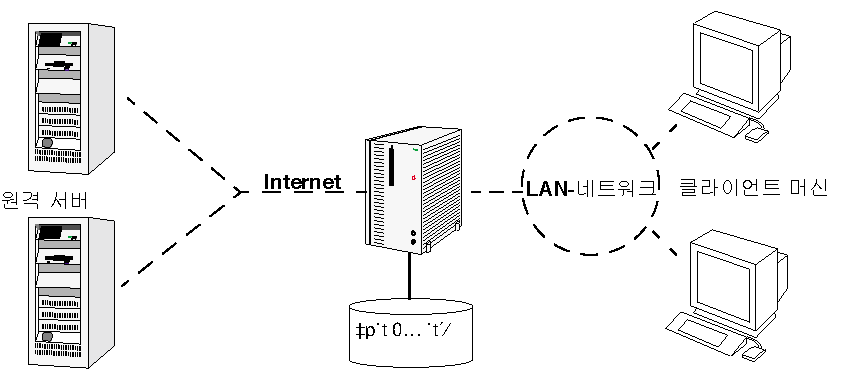
\includegraphics[width=\textwidth]{ArchitectureDiagram}
\caption{유지보수자와의 토론에서 유추한 아키텍처 다이어그램}
\figlabel{ArchitectureDiagram}
\end{center}
\end{figure}

사무실로 돌아와서 로컬 서버를 테스트하기 위한 명령 순서와 자동 거래 처리 및 여러 통화로 결제하기 위한 사용 시나리오가 포함된 간단한 보고서를 작성한다. 보고서에는 아키텍처 다이어그램(그림 6)과 다음과 같은 관찰 사항도 포함된다.

\begin{bulletlist}
  \item 인터넷 프로토콜 테스트는 수동으로 수행하여 회귀 테스트(regression test)에 대해 조사한다.

  \item 인터넷 프로토콜 사양은 독일 의료 보험 컨소시엄에서 제공받았다.

  \item 환자 목록 정렬해보고, 성 대신 이름 기준으로 정렬되는 것을 알았다.
\end{bulletlist}

\subsection*{근거}

\index{베넷, 사이몬}
\begin{quotation}
\noindent
\emph{``인터뷰 대상자의 답변에 유연하게 대응할 수 있는 능력은 인터뷰가 널리 사용되는 이유 중 하나이다.''}

\hfill --- 사이몬 베넷, \etal., \cite{Benn99a}

\index{넬슨, 제이콥}
\noindent
\emph{``인터뷰는 인터뷰 수행자가 상황에 맞게 인터뷰를 조정할 수 있기 때문에 아직 무엇을 찾고 있는지 모르는 탐색적 연구에 적합하다''}

\hfill --- 제이콥 넬슨, \cite{Niel93b}
\end{quotation}

소프트웨어 시스템을 사용하는 사람들을 인터뷰하는 것은 중요한 기능과 일반적인 사용 시나리오를 파악하는 데 필수적이다. 하지만 리엔지니어링 초기 단계에서는 무엇을 물어봐야 할지 모르기 때문에 미리 정의된 질문을 하는 것은 효과적이지 않다. 단순히 사람들이 시스템에 대해 어떤 점을 좋아하는지 물어보면 모호하거나 의미 없는 답변이 나올 수 있다. 게다가 사용자들은 레거시 시스템에 대해 불평하는 경향이 있기 때문에 매우 부정적인 답변을 얻을 위험이 있다. 

\index{골드버그, 아델}
\index{루빈, 케니}
\begin{quotation}
\noindent
\emph{``분석의 진정한 도전은 전문가가 다른 사람, 즉 분석가에게 개념을 전달해야 할 때 시작된다. 개념은 매우 풍부하고 광범위한 경우가 많기 때문에 일반적으로 전문가가 자신의 이해 전체를 하나의 총체적인 표현으로 적절하게 전달하는 것은 불가능하다.''}

\hfill --- 아델 골드버그, 케니 루빈, \cite{Gold95a}
\end{quotation}

포워드 엔지니어링 상황과 비교할 때 리버스 엔지니어는 작동 중인 소프트웨어 시스템이 있고 이를 활용할 수 있다는 한 가지 큰 장점이 있다. 이러한 상황에서는 데모를 요청하여 사용자에게 주도권을 넘기는 것이 안전하다. 우선, 데모를 통해 사용자는 자신의 말로 이야기를 전달할 수 있지만 데모는 일종의 유형적 구조를 부과하기 때문에 이해할 수 있다. 둘째, 사용자는 작동하는 시스템에서 시작해야 하기 때문에 무엇이 작동하는지 보다 긍정적인 태도로 설명할 수 있다. 마지막으로, 데모를 진행하는 동안 면접관은 정확한 질문을 많이 하고 정확한 답변을 얻을 수 있으므로 시스템 사용법에 대한 전문 지식을 파악할 수 있다.

\subsection*{알려진 용도}

이 패턴의 주요 아이디어인 사용자가 시스템을 사용하는 동안 시스템을 설명하게 하는 것은 일반적으로 사용자 인터페이스를 평가하는 데 사용된다. ``소리 내어 생각하기(Thinking aloud)는 가장 가치 있는 사용성 엔지니어링(usability engineering) 방법일 수 있다. 기본적으로 소리 내어 생각하기 테스트는 피험자가 지속적으로 큰 소리로 생각하면서 시스템을 사용하도록 하는 것이다.'' \cite{Niel93b} 요구사항 도출(requirements elicitation)을 위한 신속한 프로토타입 제작에도 동일한 아이디어가 종종 적용된다 \cite{Somm96a}.

\ind{FAMOOS} 프로젝트 초기의 한 일화에서는 이 패턴의 변형인 \variant{자신에게 직접 시연하기}를 적용하여 소프트웨어 시스템이 작동하는 것을 보고 무지한 질문이 어떻게 유지보수 팀 내에서 잠자고 있는 전문성을 촉발할 수 있는지를 보여준다. 사례 연구 중 하나인 데이터베이스 계층, 도메인 객체 계층, 사용자 인터페이스 계층으로 구성된 3계층 시스템(3-tiered system)의 전형적인 예로 '비즈니스 객체를 가져와야 한다'는 요청을 받았다. 두 명의 개인에게 이 작업을 맡겼는데, 한 사람은 소스 코드 브라우저와 CASE 도구를 사용하여 해당 비즈니스 객체를 나타내는 클래스 다이어그램을 추출했다. 다른 한 명은 로컬 PC에 시스템을 설치하고 약 한 시간 동안 사용자 인터페이스를 가지고 놀면서(즉, 시스템을 직접 시연하면서) 자신이 관찰한 몇 가지 이상한 점에 대한 10가지 질문 목록을 작성했다. 그 후, 시스템의 수석 분석가-설계자와 시스템을 리버스 엔지니어링하려고 시도한 두 사람과 함께 회의가 진행되었다. 분석가-설계자는 클래스 다이어그램을 보고 이것이 실제로 비즈니스 객체라는 것을 확인했지만, 뭔가 빠진 것이 있는지, 설계의 근거가 무엇인지에 대해서는 말해주지 않았다. 우리가 10가지 질문을 던지고 나서야 그는 설계 과정에서 직면한 문제에 대해 매우 열정적이고 매우 상세한 설명을 시작했고, 심지어 이야기 도중 클래스 다이어그램을 가리키기도 했다! 분석가 겸 디자이너의 이야기를 듣고 나서 소스코드에서 클래스 다이어그램을 추출한 사람의 첫 반응은 '이런, 소스코드에서 그런 걸 읽은 적이 없다'는 것이었다.

\subsection*{관련 패턴}

최종 사용자와 상호 작용하는 방법에 관한 많은 좋은 조언이 ``고객 상호 작용 패턴(Customer Interaction Patterns)'' \cite{Risi00a}에 구체화되어 있다. 이 패턴의 주요 메시지는 ``판매가 아닌 관계(It's a Relationship, Not a Sale)''라는 것으로, 최종 사용자와의 접점에서 신뢰 관계를 구축하는 것을 목표로 해야 한다는 점을 강조한다.

\subsection*{다음 단계}

최적의 결과를 얻으려면 여러 종류의 사람들과 \patref{데모 중 인터뷰하기}{InterviewDuringDemo}를 여러 번 시도해야 한다. 취향에 따라 이러한 시도를 \patref{한 시간 안에 모든 코드 읽기}{ReadAllTheCodeInOneHour} 및 \patref{문서 스키밍하기}{SkimTheDocumentation}의 전, 후 또는 혼합하여 수행할 수 있다. 그 후에는 \patref{유지보수자와 담소나누기}{ChatWithTheMaintainers}를 사용하여 일부 결과를 확인한다. 

시스템과의 첫 접촉이 끝나면 프로젝트를 어떻게 진행할지 (또는 취소할지) 결정해야 한다. 데모를 보면 사람들이 시스템을 어떻게 사용하는지, 어떤 기능을 높이 평가하는지에 대한 느낌을 알 수 있다. 따라서 소프트웨어 시스템의 중요한 부분과 리버스 엔지니어링이 필요한 부분을 알 수 있다. 사용 시나리오는 \patpgref{디자인에 대해 추측}{SpeculateAboutDesign} 및 \patpgref{비즈니스 규칙을 테스트로 기록}{RecordBusinessRulesAsTests}와 같은 패턴의 입력으로도 사용할 수 있다.

%=================================================================
%:PATTERN -- Do a Mock Installation
\pattern{모의 설치 수행하기}{DoAMockInstallation}

\intent{시스템을 설치하고 코드를 다시 컴파일하여 필요한 산출물을 사용할 수 있는지 확인한다.}

\subsection*{문제}

시스템을 (재)빌드할 수 있다는 것을 어떻게 확신할 수 있는가?

\emph{이 문제는 다음과 같은 이유로 어렵다.}

\begin{bulletlist}
  \item 여러분에게는 시스템이 새롭기 때문에 시스템을 빌드하는 데 필요한 파일을 모른다.

  \item 시스템이 라이브러리, 프레임워크, 패치에 의존할 수 있으며 올바른 버전을 사용할 수 있는지 확실하지 않다.

  \item 시스템이 크고 복잡하며 시스템이 실행되는 정확한 구성이 불분명하다.

  \item 유지보수자가 이러한 질문에 답하거나 설명서에서 답을 찾을 수 있지만 이 답변이 완전한지 확인해야 한다.
\end{bulletlist}

\emph{그러나 이 문제를 해결할 수 있는 이유는 다음과 같다.}

\begin{bulletlist}
  \item \emph{소스 코드(source code)}와 필요한 빌드 도구(예: 메이크파일, 컴파일러, 링커)에 접근할 수 있다.

  \item 실행 중인 시스템과 유사한 환경(예: 설치 CD 및 올바른 운영 체제가 설치된 컴퓨터)에서 시스템을 \emph{재설치(re-install)}할 수 있다.

  \item 시스템에 일종의 \emph{자체 테스트(self test)}가 포함되어 있을 수 있다. (\charef{테스트라는 생명 보험}{TestsYourLifeInsurance} 참조)를 사용하여 빌드 또는 설치가 성공했는지 확인할 수 있다.
\end{bulletlist}

\subsection*{솔루션}

제한된 시간(최대 하루) 동안 깨끗한 환경에서 시스템을 설치 및 빌드해 보자. 시스템에 자체 테스트가 포함되어 있으면 실행한다. 

\subsubsection*{힌트}

설치 및 빌드 프로세스를 완전히 이해하는 것이 아니라 다시 수행할 수 있는지 확인하는 것이 핵심이다.

빌드 및 설치 프로세스 중에 발생하는 모든 작은 오류와 해결 방법을 기록하면 시스템 구성과 라이브러리, 프레임워크 및 패치에 대한 종속성에 대해 알 수 있으므로 이를 기록하자. 예를 들어 특정 위치에서 시스템을 컴파일할 수 없거나 특정 컴퓨터에서만 액세스할 수 있는 오래된 레거시 라이브러리가 필요하거나 특정 라이브러리 패치가 필요하다는 사실을 알게 될 수 있다.

결국 시스템을 완전히 빌드하거나 설치하는 데 성공하지 못했을 수도 있다. 이는 리엔지니어링 프로젝트에 큰 영향을 미칠 가능성이 높은 위험에 해당하므로 계속 진행하기 전에 빌드 및 설치 절차를 연구하고 필요한 경우 이를 조정할 계획을 세워야 한다.

이 빌드 및 설치 실험이 끝나면 다음 내용이 포함된 보고서를 준비하자.

\begin{bulletlist}
  \item 사용된 라이브러리, 프레임워크 및 패치의 \emph{버전(version number)}

  \item 인프라(데이터베이스, 네트워크 툴킷, 포트, $\cdots$) 간의 \emph{종속성(dependency)}.

  \item 발생한 \emph{문제(problem)}와 해결 방법.

  \item \emph{개선(improvement)}에 대한 제안 사항.

  \item (불완전한 설치 또는 빌드의 경우) 솔루션 및 해결 방법의 가능성을 포함한 상황에 대한 \emph{평가(assessment)}.
\end{bulletlist}

\subsection*{트레이드오프}

\subsubsection*{장점}

\begin{bulletlist}
  \item \emph{필수 전제 조건.}
시스템을 (재)구축하거나 (재)설치할 수 있는 능력은 리엔지니어링 프로젝트에 필수적이므로 이 문제를 초기에 평가해야 한다. 구축 또는 설치가 어렵거나 불가능한 것으로 판명되면 필요한 수정 조치를 계획하자.

  \item \emph{정확성 요구.}
빌드 및 설치 프로세스를 복제하면 필요한 구성 요소에 대해 정확하게 파악해야 한다. 특히 마이그레이션 프로젝트의 경우 모든 구성 요소를 대상 플랫폼에서도 사용할 수 있어야 하므로 이 정보는 매우 중요하다.

  \item \emph{신뢰성을 높이기.}
빌드 또는 설치 후에는 어려운 단계를 직접 경험하게 된다. 개선에 대한 구체적인 제안을 쉽게 할 수 있어야 유지 관리 팀에 대한 신뢰도가 높아질 것이다.
\end{bulletlist}

\subsubsection*{단점}

\begin{bulletlist}
  \item \emph{지루한 활동.}
특히 대부분의 문제가 지금은 관심이 없는 사소한 세부 사항에 달려 있기 때문에 시스템 설치 실패의 원인을 추적하는 동안 매우 비생산적으로 느껴질 것이다. \patref{모의 설치 수행하기}{DoAMockInstallation}에 할애하는 시간을 제한하면 이 효과를 어느 정도 줄일 수 있지만, 그러면 시스템 구축이나 설치에 성공하지 못했기 때문에 더욱 비생산적으로 느껴질 것이다.

  \item \emph{불확실성.}
이 패턴은 정밀성을 요구하지만 일부 구성 요소를 재설계한 후 실제로 시스템 구축에 성공할 수 있다는 보장은 없다. 특히 신뢰할 수 있는 자체 테스트가 누락되면 빌드 또는 설치가 완료되었는지 확인할 수 없다.
\end{bulletlist}

\subsubsection*{어려움}

\begin{bulletlist}
  \item \emph{고민하지 않고 계속 시도하기.}
복잡한 시스템을 구축하거나 설치할 때 외부 요인(누락된 구성 요소, 불명확한 설치 스크립트)으로 인해 쉽게 실패할 수 있다. ``다음번에는 되겠지''라는 생각에 이런 성가신 문제를 계속 수정하고 싶은 유혹에 빠지기 쉽다. 이러한 세부 사항에 얽매이기보다는 시스템을 구축하는 것이 아니라 구축 프로세스에 대한 통찰력을 얻는다는 주요 목표를 놓치지 않는 것이 중요하다. 따라서 시간을 제한하고 발생하는 문제를 문서화하는 데 집중하여 나중에 문제를 해결할 수 있도록 해야 한다.
\end{bulletlist}

\subsection*{예시}

일부 최종 사용자와 \patref{데모 중 인터뷰}{InterviewDuringDemo}를 수행했으며, 그 결과 리엔지니어링 프로젝트에서 유지해야 할 중요한 기능에 대한 감을 잡았다. 하지만 프로젝트를 수락하기 전에 시스템을 변경할 수 있는지 여부를 확인해야 한다. 따라서 시스템을 새로 빌드할 수 있는지 확인하기 위해 간단한 실험을 해보기로 결정한다.

데이브가 사무실에 두고 간 상자에서 모든 소스 코드가 들어 있는 두 번째 CD를 가져온다. 디렉터리를 살펴보다가 최상위 메이크파일 하나를 발견하고 시도해 보기로 결정한다. 모든 파일을 시스템의 Linux 파티션에 복사하고 프롬프트에 \cmd{make all} 명령을 입력한다. 잠시 동안 모든 것이 순조롭게 진행되며 시스템은 수많은 자바 컴파일 성공을 보고한다. 하지만 안타깝게도 몇 분 후 \ct{java.sql} 라이브러리가 누락되어 make가 실패한다. JDK1.1이 설치되어 있다는 사실을 깨닫게 되지만, 문서에서 JDK1.3이 설치되어야 한다고 언급한 것을 기억한다. 마지못해 전체 디렉토리 구조를 휴지통에 버리고 JDK1.1을 제거한 다음 JDK1.3을 다운로드하여 설치한 다음(다운로드하는 데 시간이 오래 걸리므로 커피 한 잔을 가져와야 한다) 다시 시작한다. 이번에는 C 코드 컴파일이 시작될 때까지 메이크가 순조롭게 진행된다. 라이브러리 파일이 누락되어 첫 번째 컴파일이 즉시 실패하고 C 파일을 열어 이 실패의 원인이 정확히 무엇인지 확인합니다. assert.h는 시스템에서 사용할 수 있는 표준 라이브러리이므로 검색 경로에 문제가 있는 것이 분명하다. 그때는 거의 점심 시간이었고 오늘 이 빌드 실험을 끝내기로 계획했기 때문에 전체 C 컴파일은 나중에 하기로 결정했다. 어쨌든 데이브가 팀에 같이 있고, 그가 이 C 코드를 작성했으니 컴파일하는 방법을 보여줄 수 있을 것이다.

점심 식사 후에는 작성한 코드가 정상인지 확인하고 싶을 것이다. \lct{"void main("}를 grep하면 \emph{XDoctor}.java 파일에 메인 항목이 포함되어 있음을 알 수 있으므로 java \emph{XDoctor}를 입력하여 시스템을 실행한다. 실제로 데모에서 보셨던 시작 화면이 나타나고 \emph{``시스템이 데이터베이스에 연결 중입니다''}라는 작은 상태 창이 나타난다. 그 직후 \emph{``예상치 못한 일이 발생했습니다''} 메시지와 함께 시스템이 실패하고 데이터베이스 누락이 원인인 것으로 의심된다. 이 문제를 나중에 조사하기로 결정하고 설치 절차를 확인하기로 한다.

시스템을 설치할 수 있는지 확인하기 위해 설치 CD를 Macintosh의 CD 드라이브에 넣는다. 자동으로 일반적인 설치 창이 나타나고 설치 프로세스를 원활하게 진행한다. 설치 프로세스가 완료되면 설치 프로그램에서 시스템을 시작하기 전에 컴퓨터를 재부팅하라는 메시지가 표시된다. 어떤 시스템 확장 프로그램이 설치되었는지 확인하고 컴퓨터를 재부팅한 다음 바탕화면에 나타난 \emph{XDoctor} 아이콘을 더블 클릭한다. 안타깝게도 라이센스 키를 입력하라는 창이 나타납니다. CD 상자를 살펴보니 라이센스 키는 별도의 편지로 받았어야 하는데 당연히 받지 못했다. ``아쉽네, 라이선스 키가 제공되지 않았을 때 \emph{proDoc}처럼 시스템의 데모 버전을 실행할 수 있으면 좋았을 텐데'' 하는 생각이 든다. 좌절하여 포기하고 다음과 같은 보고서를 작성하기로 결정한다.

\begin{bulletlist}
  \item JDK1.3으로 make가 작동하는 것으로 보임: 이 빌드가 완료되었는지 확인할 수 없다.

  \item C 컴파일 실패: 데이브에게 빌드 데모를 요청한다.

  \item 라이선스 더 자세히 조사: 시스템이 어떻게 보호되는가?

  \item \emph{제안:}
라이선스 키가 제공되지 않으면 데모 모드로 실행한다(참조: \emph{proDoc}).

  \item \emph{제안:}
호출 시 사전 조건을 확인한다. \ct{XDoctor.main()}; 새로 빌드한 후 ``예기치 않은 일이 발생했다''라는 메시지와 함께 시스템이 종료된다.
\end{bulletlist}

\subsection*{알려진 용도}

\ind{FAMOOS} 사례 연구 중 하나에서는 중앙 서버와 소켓을 통해 통신하는 분산 시스템을 간단한 명령어를 사용하여 리엔지니어링해야 했다. 첨부된 편지에 따르면 ``필요한 모든 것이 들어 있는'' tar 파일이 들어 있는 테이프를 받았다. 그러나 시스템을 재구축하고 다시 설치하는 것이 어려웠고, 설치 스크립트를 자세히 살펴보고 관리자에게 설명을 요청해야 했다. 결국 보안 및 연결 문제로 인해 중앙 서버와 통신할 수는 없었지만 시뮬레이션 모드에서 시스템을 테스트할 수 있었다. 실험이 완전히 성공하지는 못했지만 시스템 아키텍처에 대한 인사이트를 얻을 수 있었다. 특히 시뮬레이션 모드가 중앙 서버를 모방하는 방식과 이것이 소스 코드와 메이크파일에 인코딩되는 방식은 나머지 프로젝트 기간 동안 중요한 정보를 제공했다.

우리가 수행한 감사 프로젝트의 첫날이 끝날 무렵, 다음 날 아침 새로 설치한 것을 보여 달라고 요청했다. 저희는 이를 \patref{데모 중 인터뷰하기}{InterviewDuringDemo}를 위한 준비를 위한 순수한 요청이라고 생각했지만, 설치 도중 한 명의 관리자가 설치 CD를 준비하기 위해 밤을 새워야 했다는 사실을 알게 되었다. 그 후의 토론을 통해 우리는 이 시스템이 사용자 기반이 고정되어 있고 인터넷을 통해 매주 업데이트를 다운로드하도록 설계된 시스템이라는 사실을 알게 되었다. 이는 이전에 \patref{한 시간 안에 모든 코드 읽기}{ReadAllTheCodeInOneHour}를 위해 노력하는 동안 관찰한 많은 특이한 점을 설명해 주었고, 남은 감사 프로젝트 동안 설계 문제를 드러내는 데 많은 도움이 되었다.

구성 관리 시스템(configuration management system)으로 작업할 때는 코드를 다시 컴파일하기 전에 먼저 코드를 깨끗한 구성으로 가져오는 것이 좋다. 예를 들어 \ind{Smalltalk} 시스템의 경우, 시스템을 구성하는 \ind{Envy} 구성 맵을 먼저 로드한 다음 코드를 깨끗한 이미지로 로드하는 것이 일반적인 조언 중 하나이다 \cite{Pelr01a}. 

\subsection*{다음 단계}

결론을 보고하기 전에 \patref{유지보수자와 담소나누기}{ChatWithTheMaintainers}를 하는 것이 좋다. 유지보수자는 여러분의 조사 결과를 확인하고 오해를 풀 수 있을 것이다. 개선에 대한 구체적인 제안은 관리자와 논의하는 것이 가장 좋은데, 이는 여러분이 진정으로 그들을 돕고자 하는 의지가 있음을 설득할 수 있는 가장 좋은 방법이기 때문이다.

빌드 또는 설치가 완전히 실패하는 경우 \patref{데모 중 인터뷰하기}{InterviewDuringDemo}를 \patref{모의 설치 수행하기}{DoAMockInstallation}와 결합하는 것이 좋다. 이 경우 유지보수자에게 빌드 또는 설치 프로세스를 시연해 달라고 요청하고 불분명한 단계에 대해 질문하자.

%=============================================================
\ifx\wholebook\relax\else
   \bibliographystyle{alpha}
   \bibliography{scg}
   \end{document}
\fi
%=============================================================
